%%%%%%%%%%%%%%%%%%%%%%%%%%%%%%%%%%%%%%%%%%%%%%%%%%%%%%%%%%%%%%%%%%%%%%%%%%%%%%%
\documentclass[11pt]{article}
\usepackage{graphicx,times,lscape,fancyheadings,color}

\textwidth 6.5in
\textheight 9.0in
\oddsidemargin -0.1in
\topmargin -0.5in
\parindent 0.0in
\parskip 5pt

\setcounter{secnumdepth}{4}

\chead{}
%%%%%%%%%%%%%%%%%%%%%%%%%%%%%%%%%%%%%%%%%%%%%%%%%%%%%%%%%%%%%%%%%%%%%%%%%%%%%%%%
% spindle2 specific latex macros
% 2006/08/10

%% Requirements

\newcommand{\refreq}[1]{Requirement~\ref{#1}}

\newtheorem{reqBlock}{REQ}[section]

\newcommand{\reqlabel}[1]{\mbox{\textsc{#1:}}\hfil}
\newenvironment{reqlist}[1]{%
  \begin{list}{}{%
      \renewcommand{\makelabel}{\reqlabel}%
      \settowidth{\labelwidth}{\mbox{\textsc{#1:}}}%
      \setlength{\leftmargin}{\labelwidth+\labelsep}%
    }\itemsep=0pt\parsep=0pt\parskip=0pt}{%
  \end{list}%
}
\newcommand{\req}[2]{%
  \begin{reqBlock}
    #1%
\ifx#2\empty\else%
\begin{reqlist}{Description}
  #2
\end{reqlist}
\fi
\end{reqBlock}
}
\newcommand{\reqSrc}{\item[Source]}
\newcommand{\reqQuote}{\item[Quote]}
\newcommand{\reqYear}{\item[Year]}
\newcommand{\reqWhen}{\item[When]}

\newcommand{\phase}[1]{\textbf{$\mathbf{[}$\textsc{Phase #1}$\mathbf{]}$}}

% Macros for interface message/primitive definitions. Originally from
% ADROIT, fixed by clivadas

\newcommand{\metlabel}[1]{\mbox{\textsc{#1}}\hfill}
\newcommand{\metP}{\item[Parameters]}
\newcommand{\metD}{\item[Description]}
\newcommand{\metM}{\item[DTN2 $\Delta$]}
\newcommand{\metR}{\item[Related]}

\newcommand{\method}[2]{%
\noindent
\textbf{#1}
\begin{list}{}%
  {\renewcommand{\makelabel}{\metlabel}%
    \settowidth{\labelwidth}{\mbox{\textsc{OutputXXXXX}}}%
    \setlength{\leftmargin}{\labelwidth}%
    \addtolength{\leftmargin}{\labelsep}%
  }
  #2
\end{list}
\vspace{0.15in}
}


%%%%%%%%%%%%%%%%%%%%%%%%%%%%%%%%%%%%%%%%%%%%%%%%%%%%%%%%%%%%%%%%%%%%%%%%%%%%%%%
\begin{document} 

\title{DTN Plugin Architecture \\
{\large Approved for Public Release, Distribution Unlimited.  [2/27/2007]}
} 

\author{Rajesh Krishnan, Christopher Small, Ram Ramanathan, Joanne Mikkelson, 
and Prithwish Basu\thanks{Contact: pbasu@bbn.com, 617.873.7742}\\ 
BBN Technologies, 10 Moulton St, Cambridge MA 02138} 
\date{\today}
\maketitle

\tableofcontents
%%%%%%%%%%%%%%%%%%%%%%%%%%%%%%%%%%%%%%%%%%%%%%%%%%%%%%%%%%%%%%%%%%%%%%%%%%%%%%%
\newpage
\section{Introduction} \label{sec:intro}

In this document, we describe a DTN reference system architecture.  The purpose
of this document is to identify the components of the DTN reference system, 
and to define and specify the semantics of the interfaces between the 
components.  
%We seek feedback from the DTN community on the architecture and
%the interfaces described here, for possible inclusion in future versions of
%this document.

The reader is assumed to be familiar with the Bundle Protocol
specification~\cite{BP-ID}, the Bundle Security Protocol
specification~\cite{BSP-ID}, and the DTNRG reference
implementation~\cite{DTN2}.  

A particular goal of this architecture is to enable the community to experiment
with multiple solutions for persistent storage, routing, naming and late
binding, policy, and DTN convergence layers, while continuing to build upon a
common core of open DTNRG standards and software. This is accomplished by
defining interfaces that allow the experimental features to plug into the
common core.  In this document, the term {\em system} will refer to the
SPINDLE-II DTN system (the core of which is based on the DTN2 system), unless
specified otherwise.  

\subsection{Glossary of Abbreviations and Technical Terms} \label{sec:glossary}

Some commonly used acronyms and terms used throughout this document are listed
and described below.

\begin{description}
\item[A/M] Application / Middleware
\item[BPA] Bundle Protocol Agent
\item[BP] Bundle Protocol
\item[BSP] Bundle Security Protocol
\item[CLA] Convergence Layer Adapter
\item[DBMS] Database Management System
\item[DP] Decision Plane
\item[DS] Data Store
\item[DTNRG-public] A design specification that will undergo the DTNRG consensus process during DTN Program Phase 2.
\item[EID] Endpoint IDentifier for denoting a DTN endpoint (see~\cite{BP-ID})
\item[GBOF-ID] Global Bundle Or Fragment ID
\item[KB] Knowledge Base
\item[Link] An association between two DTN endpoints (detailed description in Section \ref{sec:linktypes})
\item[MANET] Mobile Ad hoc NETwork
\end{description}

%%%%%%%%%%%%%%%%%%%%%%%%%%%%%%%%%%%%%%%%%%%%%%%%%%%%%%%%%%%%%%%%%%%%%%%%%%%%%%%
\newpage
\section{Overview} \label{sec:complist}

The high-level components and interfaces of the system are illustrated in 
Figure \ref{fig:componly}.

%%%%%%%%%%%%
\begin{figure}[htbp]
\centering
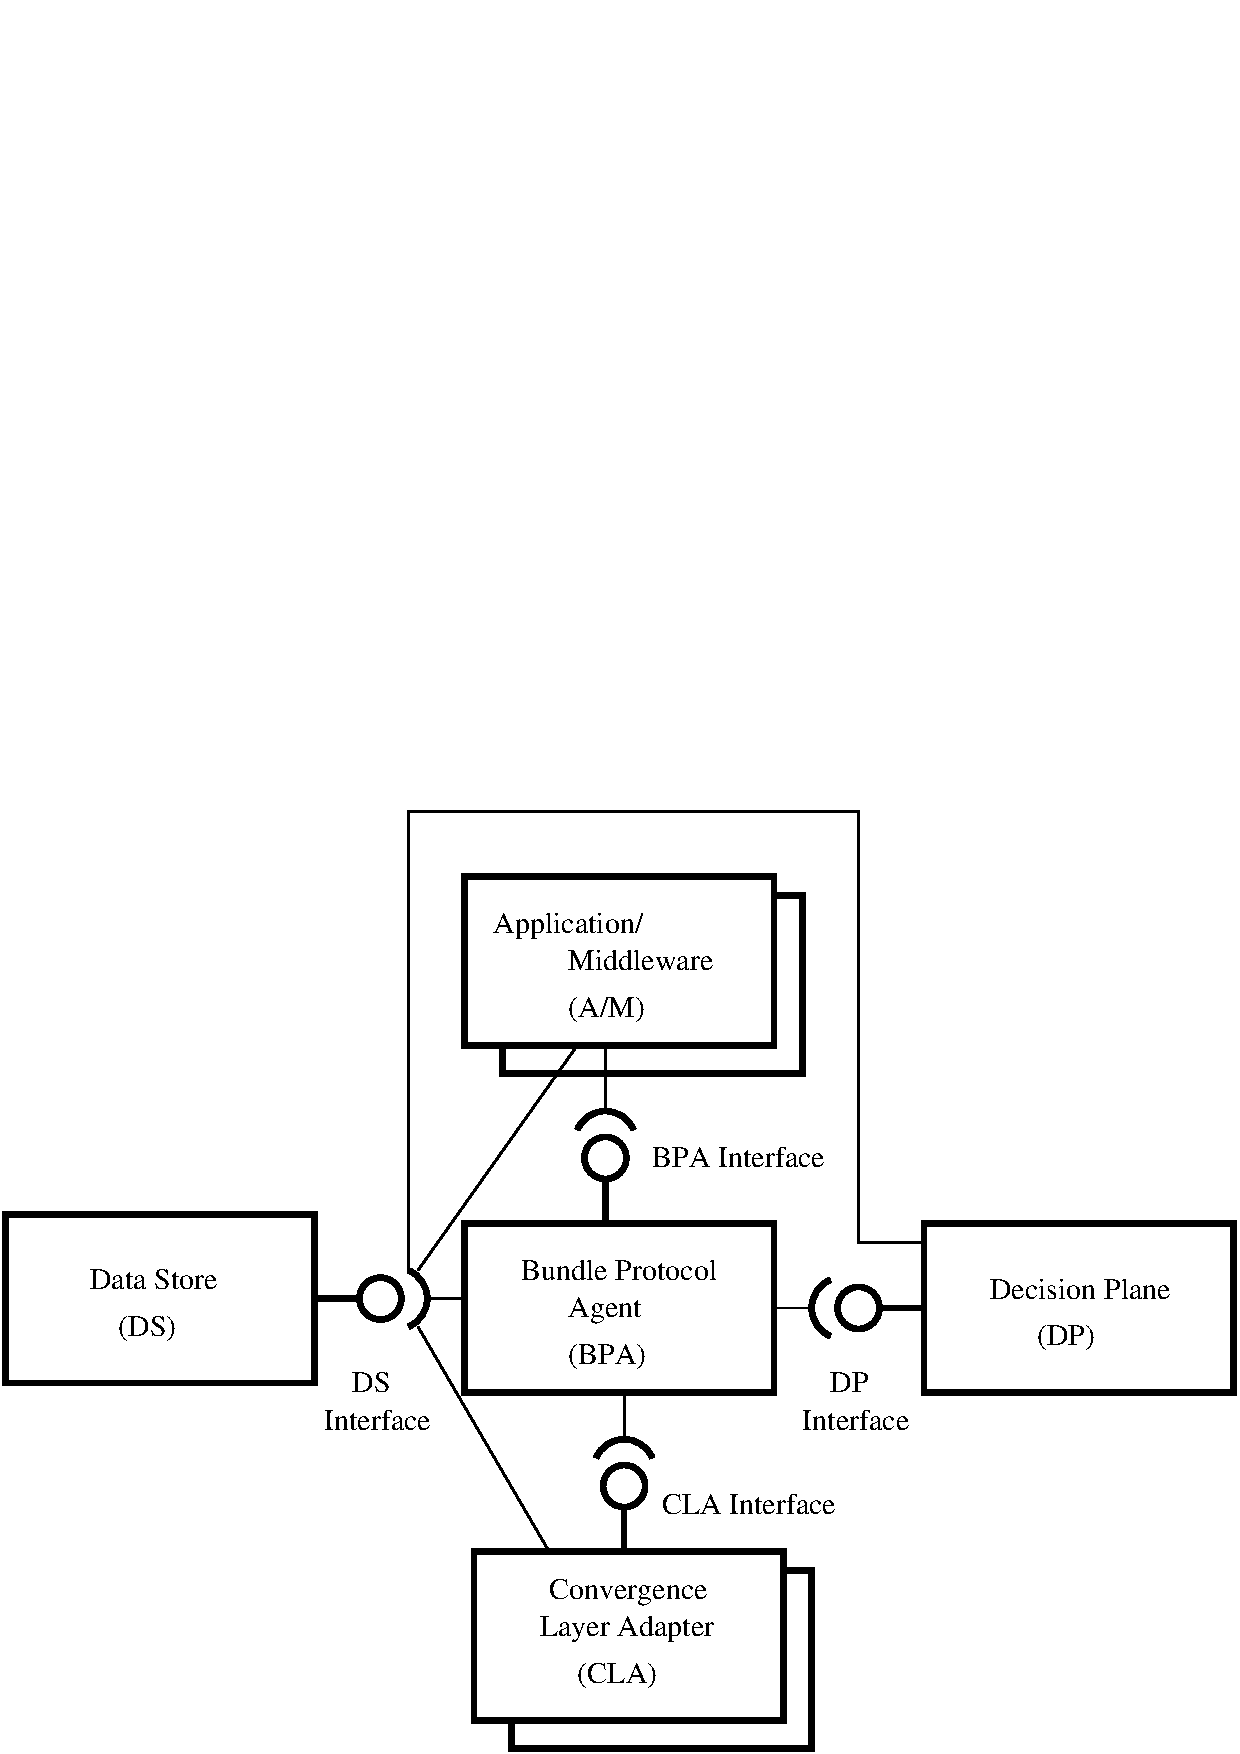
\includegraphics[height=3in]{figs/components-toplevel.pdf}
\caption{\label{fig:componly} Architectural Components and Interfaces}
\end{figure}
%%%%%%%%%%%%
%

The system SHOULD contain the following components (described in
Section \ref{sec:compdesc}):

\vspace{-4pt}
\begin{enumerate}
\setlength{\parskip}{-3pt}
\item Bundle Protocol Agent (BPA), a DTNRG-public component
\item Data Store (DS)
\item Decision Plane (DP)
\item Convergence Layer Adapter (CLA)
\item Application/Middleware (A/M)
\end{enumerate}

Table \ref{tab:comp-functions} summarizes the key functionality provided by
each of the five components. The above components MAY be implemented in
separate processes to enable language and tool-chain independence across
components. 

Instances of the BPA will be also referred to as the {\it core} and instances
of the other four components shall be referred to as {\it plugins}.  The DS
SHOULD provide a service that is accessible from all other components of the
system.\footnote{As a result, the system can support both daemon-centric and
database-centric concepts of operation.}

The system MUST implement the relevant DTNRG-public interfaces as name below
and described in Section \ref{sec:interfaces}:
\vspace{-4pt}
\begin{enumerate}
\setlength{\parskip}{-3pt}
\item Data Store Interface (used by BPA, CLA, DP, and A/M)
\item Decision Plane Interface (used by BPA)
\item Convergence Layer Adapter Interface (used by BPA)
\item Bundle Protocol Agent Interface (used by A/M)
\end{enumerate}

All interfaces SHOULD be provided using the Inter-Component Communication 
protocol (discussed in Section \ref{sec:iccp}, defined in a separate document)
for uniformity.

%%%%%%%%%%%%%%%%%%%%%%%%%%%%%%%%%%%%%%%%%%%%%%%%%%%%%%%%%%%%%%%%%%%%%%%%%%%%%%%
\begin{landscape}
\begin{table}[htbp]
\centering
{\small
\begin{tabular}{|p{1.5in}|p{1.5in}|p{1.5in}|p{1.5in}|p{1.5in}|}
\hline
{\bf BPA} & {\bf DS} & {\bf CLA} & {\bf DP} & {\bf A/M}\\
\hline
Implement the Bundle Protocol specification
&
Store, retrieve, and delete key-data pairs
&
Provide a bundle transport mechanism
&
Receive link and bundle event notifications from the BPA and 
generate actions (requests).
&
Generate, submit, and receive application bundle payloads
\\
\hline

Implement the Bundle Security Protocol specification
&
Database management for metadata, including schema management,
and query processing
&
Neighbor discovery (via scanning or staring)
&
Provide an adaptive dissemination service that can be used 
by various routing and naming protocols
&
Create/remove registration with BPA
\\
\hline

Implement the Bundle Protocol Agent Interface (accessed by A/M)
&
Knowledge base management for metadata, including ontology management,
query processing, and rule-based inference
&
Link formation, tear-down, and characterization (e.g., delay, capacity, 
loss) 
&
Perform a long-term characterization of available communication 
opportunities (e.g., computes a cost metric)
&
Register procedure(s) for handling delivery failure
\\
\hline

Use and implement support for DP interface, CLA interface, and DS interface
&
Manage storage of bundles, bundle metadata, registration information, BPA state
if any, connectivity (historic, current, and scheduled) information, naming
ontology, and cached content 
&
Link status reporting (e.g., in response to queries)
&
Process policy inputs and respond to queries regarding decision choices
that conform to policy
&
\\
\hline

&
Database triggers
&
Implement CLA interface
&
Perform forwarding and scheduling decisions for bundles
&
\\
\hline

&
Implement DS interface
&
&
Perform route computation and/or route discovery
&
\\
\hline

&
&
&
Perform name resolution and distributed name KB management
&
\\
\hline

&
&
&
Implement DP interface
&
\\
\hline

\end{tabular}
}
\caption{Summary of functionality of system components \label{tab:comp-functions}}
\end{table}
\end{landscape}

%%%%%%%%%%%%%%%%%%%%%%%%%%%%%%%%%%%%%%%%%%%%%%%%%%%%%%%%%%%%%%%%%%%%%%%%%%%%%%%
\newpage
\section{Architectural Components} \label{sec:compdesc}

In this section we describe each of the system components mentioned in Section
\ref{sec:complist} (DS, CLA, DP, A/M). These will be implemented as plug-ins in
the SPINDLE-II system; in other words, a newly developed module (implemented as
a process) can be started on the node and its services will be automatically
available to the other already running DTN processes.


%%%%%%%%%%%%%%%%%%%%%%%%%%%%%%%%%%%%%%%%%%%%%%%%%%%%%%%%%%%%%%%%%%%%%%%%%%%%%%%
\subsection{Bundle Protocol Agent}
\label{sec:bpa}

The bundle protocol agent (BPA) of a DTN node offers bundle protocol (BP)
services.  The BPA executes procedures of the BP and the Bundle Security
Protocol (BSP) with help from other components in the system.  The BPA MUST
comply with the DTNRG specifications for the BP~\cite{BP-ID} and the BSP
~\cite{BSP-ID}.  

The BPA is responsible for implementing the mechanisms of the bundle protocol,
but any key decisions (for example, those based on particular policies or
optimization strategies) that need to be taken during the execution of such
mechanisms MAY be exported to the {\em Decision Plane (DP)} module.  Typically
these decisions are indicated within the BP and BSP specifications as local
policy or implementation issues.

The BPA is responsible for taking actions on every bundle that passes through 
the DTN node.   For example, the BPA is responsible for reading, creating, 
and updating fields in the bundle header.

A comprehensive list of functional requirements for the BPA in terms of
conformance to the BP and BSP can be found in a companion document \cite{MJ}.
Some key functions are:

\begin{enumerate}

\item Forwarding a bundle to a ``next-hop'' node via a specified convergence
layer adapter.  The BP specification talks about forwarding to the ``minimum
reception group'' for each bundle in each of the unicast, multicast, and
anycast scenarios. The DP must compute these lists and returns them to the BPA
along with scheduling instructions to handle ``Class of Service'' requirements.

\item Fragmentation and reassembly of bundle payload (both reactive and 
pro-active).

\item Implementation of the Custody-transfer mechanism in the bundle header,
sending Custody Acknowledgments, etc.: The decision of whether to accept,
refuse, or relinquish custody is taken by the DP. Once a decision has been
made, a list of DP-specified actions such as re-forwarding the bundle may have
to be taken (depends on policy).

\item Delivery to application: Deliver incoming bundle to application if it is
{\it registered} on this node; otherwise abandon delivery based on policy.

\item Discarding and Deleting a bundle: If the set of ``retention
constraints'' on a bundle is empty, then discard the bundle and all references
to it. Deleting a bundle involves removing all retention constraints and then
discarding it.  This may happen upon bundle expiration. These mechanisms can
richly interact with the policy module within the DP.

\item Sending administrative bundles such as status reports.

\item Security functions such as authentication, confidentiality, 
and data integrity.
%prevention of DOS over resource strapped networks.
\end{enumerate}

In addition, the BPA SHOULD {\it implement} the Bundle Protocol Agent Interface that
can be accessed by applications, and {\it use} the other interfaces listed in
Section \ref{sec:complist}.

%The interactions between the BPA and other components are described in 
%Section \ref{sec:XXX}.

%%%%%%%%%%%%%%%%%%%%%%%%%%%%%%%%%%%%%%%%%%%%%%%%%%%%%%%%%%%%%%%%%%%%%%%%%%%%%%%
\subsection{Data Store}
\label{sec:ds}

The Data Store (DS) module offers a persistent storage service and is
responsible for storing bundles, knowledge about bundle metadata, network state
information (routing tables, name ontology data, content metadata, policy
rules), and application state information (registrations and other metadata).
We note that the SPINDLE system may eventually need to cater to a wide spectrum
of solutions for the data storage layer. These may range from a dumb file
system residing on Flash memory attached to a low power sensor node to a very
powerful logic engine running on a powerful DTN node.  Hence a DS in the
SPINDLE system could exist in one of the following incarnations of increasing
capability: 

\begin{enumerate}
\item A simple key-value store (that can be based on a file system) that allows 
other modules to add, retrieve and delete key-value pairs. Bundles, bundle metadata 
and network state information can exist in such a store. This may be 
applicable for resource-strapped devices such as battery-powered sensor 
nodes.

\item A DBMS that allows other modules to add, delete, and get
elements with multiple fields information (by its key). An DBMS might 
expose only {\it canned queries} to other modules, or it might allow other 
modules to submit queries, e.g. written in SQL.

\item A full fledged knowledge base (KB) that supports deduction or inference
by means of execution of rules (e.g., Prolog style) on stored facts. In
addition to add/delete(key)/get(key) features, a KB will support advanced
deductive database style querying features. Advanced KBs like Flora-2 even
allow setting up ``triggers'' that fire when a certain rule executes
successfully, and this typically results in the execution of a specified
callback function.  A KB will include support for data storage, either
internally, or via a back-end storage system such as MySQL or Berkeley DB.

\end{enumerate}

%%%%%%%%%%%%%%%%%%%%%%%%%%%%%%%%%%%%%%%%%%%%%%%%%%%%%%%%%%%%%%%%%%%%%%%%%%%%%%%
\subsection{Decision Plane} \label{sec:dp}

The Decision Plane component includes the following subcomponents which may
interact with each other:

\begin{enumerate}

\item {\it Router module:} Functions of a Router module include unicast and
multicast route computation, generation of next hop(s) for bundles, replication
and forwarding, bundle scheduling, decision to take custody of a bundle,
decision to discard a bundle, etc. 

Note that while the BPA performs the forwarding mechanism to a particular CLA,
it is the Router module that performs the consulting role for the BPA.  Similarly,
for custody transfer, the BPA performs the mechanism of assuming and
relinquishing custody and sending a custody-ACK to the previous node, but it
consults the external router module to decide whether to take custody or not.

\item {\it Adaptive Dissemination module:} This is responsible for determining
{\it what} network state to distribute, and {\it to whom}, and {\it when}. It
is also responsible for gathering network state encoded in incoming
dissemination bundles and populating the KB appropriately, if one exists. For
example, decisions such as whether to alter the content of a flooded
network-state bundle before re-dissemination will be taken by this module. This
module is also responsible for interacting with CLA (via the BPA) to track
changes in the status of incoming/outgoing links and then capture these changes
in the ``to-be-disseminated'' network state.  Even though the network state is
stored in the KB, the dissemination logic may be implemented outside the KB for
performance reasons, if necessary.

\item {\it Policy module:} This will let users add and delete policies that may
be stored in the KB, if one exists. Basic functions include interpretation of
policy, enforcement of policy, and dispatching an event afterward. Performance
reasons aside, ideally every bundle or network event in the SPINDLE system
should be subjected to policy enforcement. This advocates a
``trap-and-dispatch'' (or ``event-condition-action'') style design.  An 
alternative style is that of ``consultation.'' The policy module listens on 
a well known port for policy-enforcement requests
and reacts only when asked.

\item {\it Naming and Late binding module:} This module maintains and
opportunistically shares name ontologies (or {\it schemes}, as referred to
in~\cite{BP-ID}) between DTN nodes. This module is called upon to resolve rich
intentional names to canonical endpoint identifiers of care-of nodes that are
subsequently used by the Router module. This is also responsible for
registration and dissemination or synchronization of Name KBs (in particular,
intentional name to canonical name bindings stored within).

\item {\it Content-based access module:} responsible for performing content
caching/replication, distributed indexing, and content-addressable search.
This may use several services from other DP modules, e.g., dissemination, late
binding, external router.

%{\it does this fall under Decision or App? Or maybe there should be no
%distinction?}

\end{enumerate}

%%%%%%%%%%%%%%%%%%%%%%%%%%%%%%%%%%%%%%%%%%%%%%%%%%%%%%%%%%%%%%%%%%%%%%%%%%%%%%%
\subsection{Convergence Layer Adapter}
\label{sec:cla}

A Convergence layer adapter's function (as described in \cite{BP-ID}) is to
send and receive bundles on behalf of the BPA. It achieves this by utilizing
the services of the native protocol which is supported in one of the {\it
underlying} networks that the node is homed on. A CLA thus {\it adapts} the
packet/frame/signal transmission service provided in the underlying network to
an abstract bundle transmission service that presents itself to the BPA.  

A CLA is responsible for maintaining information about DTN {\it links} (status,
schedule, and possibly other QoS parameters) and discover them if possible.
After discovering a DTN peer or monitoring the status of a link, the CLA is
responsible for generating and posting events to the BPA about such facts.
These facts then get relayed to the DP and may also be stored in the DS. 

%The CLA may also interact directly (IPC poke?) with some decision modules
%(adaptive dissemination) for triggered dissemination under certain
%circumstances. 

%{\it What is the service contract of send/receive with the BP? and how are the
%CLA params presented to BP?}

%%%%%%%%%%%%%%%%%%%%%%%%%%%%%%%%%%%%%%%%%%%%%%%%%%%%%%%%%%%%%%%%%%%%%%%%%%%%%%%
\subsection{Application/Middleware}
\label{sec:am}

The application agent (also referred to as the A/M module) uses the BP services
to transmit and receive bundle payloads. This can act as a multiplexed DTN
communication service to other non-DTN applications running on the node.

%%%%%%%%%%%%%%%%%%%%%%%%%%%%%%%%%%%%%%%%%%%%%%%%%%%%%%%%%%%%%%%%%%%%%%%%%%%%%%%
\newpage
\section{Interfaces}
\label{sec:interfaces}

In this section we describe the primitives for each of the four interfaces 
identified in Figure \ref{fig:componly}.  

The BPA implements the BPA interface that can be used by A/M and DP to send and
receive bundles.  

The DP implements the DP interface that is accessed by the BPA to serve various
decision points identified in the BP (such as routing, scheduling, name
resolution, custody acceptance, and storage management).

The DS implements the DS interface for storing bundles, bundle metadata,
application registrations, connectivity information, and other system state.
The DS interface can be accessed system-wide.  The CLA, for example, may access
the DS interface for storing and retrieving connectivity information that is
discovered or scheduled/specified.  The DP, for example, may access the DS
interface for storing and retrieving information related to routing, naming,
policy, and content caching/indexing.

The CLA implements the CLA interface which is accessed by the BPA for 
bundle transport and link management.

We briefly discuss at the end of this section the Inter-Component 
Communication Protocol (ICCP), the details of which will be described 
in a separate document.

\subsection{Interface Conventions}

We note that this is a ``semantic'' interface, that is, we expect it to be
specifying the kinds of things that go across the interface and their meanings,
not necessarily at a level necessary for implementation. We expect, though,
that an implementation-level specification can be generated from this easily.

All messages are assumed to be transparently reliably delivered.  This
functionality may be provided by the inter-component communication protocol
mentioned in Section \ref{sec:iccp}.

All parameters are assumed to be ``required'' unless specifically
noted to be ``optional'' (Opt).

The interface messages are named in a top-down hierarchical
fashion. For example, in the DP and CLA interfaces, at the highest
level, there are four kinds of messages: Event, Request, Query,
Report. At the next level, there are Link-specific and Bundle-specific
messages, for each message type. At a further level, there is
Created/Deleted, Transmitted/Received etc. which are 
the next level down.  This naming convention is intended for readability 
of the specification only. The implementation should adopt/retain the style
most convenient to it.

Query/Report messages consist of a set of ``paired'' messages---a Query
message from a plugin to the BPA requesting certain information from the BPA
and a report message (for that query) from the BPA to the plugin delivering the
requested information, if possible.\footnote{Note that Query/Report messages are
possible in the reverse direction as well, e.g., the BPA can send a Query
message to the CLA or the DS and can expect a Report back.} Unlike the
Request-Event messages which are only loosely tied, there is a tighter coupling
between query and report; in particular, a report identifies which query is
being responded to.

\subsubsection{Links and Link Types} \label{sec:linktypes}

A link in DTN2 is an association between two DTN endpoints. In other words it
can be represented as a relation between two EIDs which is established over a
certain convergence layer. A link possesses physical attributes such as
datarate, (estimated) delay, error rate, loss rate etc. as well as other
attributes including {\it type}, {\it state}, and other {\it flags}.  A 
measurement process (in the convergence layer adapter) can track and 
update the values of these attributes.

\begin{table}
\centering
\begin{tabular}{|l|c|c|c||c|c|}
\multicolumn{1}{c}{ } & \multicolumn{3}{c}{States} & \multicolumn{2}{c}{Flags} \\
\hline
Link Type & OPEN, BUSY & UNAVAILABLE & AVAILABLE & UNUSABLE & REACHABLE\footnotemark \\
\hline
Persistent (AlwaysOn)             & x & x &   & x &  \\
\hline
On-demand            & x & x & x & x &  \\
\hline
Opportunistic (Discovered)           & x & x &   & x & x\\
\hline
Scheduled            & x & x & x & x & x\\
\hline
Predicted            & x & x &   & x & x\\
\hline
\end{tabular}
\caption{\label{table:link-tsf} Link types and possible states/flags.}
\end{table}
\footnotetext{Anticipated changes in the way bundle queuing is done for 
closed links might make the REACHABLE flag unnecessary. Thus this column 
is likely to disappear in future versions.}

There are three link types implemented in DTN2: Persistent (AlwaysOn),
On-demand, and Opportunistic (Discovered).\footnote{DTN2 uses AlwaysOn
to denote what the DTN Architecture refers to as Persistent;
``Discovered'' is influenced by the term   
``neighbor discovery'' commonly used in mobile ad hoc networking literature.}
We extend the semantics of the Opportunistic link to support a wider range 
of neighbor discovery procedures.  We add the
remaining two types discussed in the DTN Architecture: Scheduled, and
Predicted.\footnote{
There is a Scheduled link type in DTN2 but it is not fully implemented.}
Not all link states and flags apply to all link types.\footnote{In
particular, note that there is no discovery for on-demand links, and
reachability is assumed.} Table \ref{table:link-tsf} depicts the various {\it
types} of links and their corresponding range of {\it states} and {\it flags}
that SHOULD be allowed in a DTN system. A detailed description of the various
link states and flags can be found in Section \ref{sec:linkstates}.

A Persistent (AlwaysOn) link is simply a static link, and it should always 
be open. The
link is opened as soon as it is created. If the link closes for any reason the
link becomes UNAVAILABLE and the BPA will attempt to reopen the link.
An example of an AlwaysOn link would be a wired connection to a peer such as a
T1. 

An On-demand link is assumed to be usable at any time as required, but is not
opened until there are bundles to be sent over the link. When in this state,
the link is AVAILABLE. Once the link is OPEN, if no bundle traffic is sent over
an on-demand link for a while, the BPA will consider the link idle and
automatically close the link, returning it to AVAILABLE. If the link closes for
any reason other than being idle or being explicitly closed by an operator, the
link becomes UNAVAILABLE and the BPA will periodically attempt to reopen the
link. If the link is successfully reopened, the link state returns to OPEN. A
dial-up connection over a modem would be represented by an
on-demand link.

An Opportunistic (Discovered) link is used with CLAs when there is no need 
to form a {\em point-to-point} connection for a link to be open.   
Discovered links are intended to capture characteristics of communications in 
multihop broadcast wireless networks (MANETs). Note that
in a broadcast channel context there really is no ``link'' {\it per se,} but peers
discover ability to communicate, which we declare as links. 
%We shall assume, as
%is consistent with current state of art, that the CLA only discovers and
%uses two-way communication possibilities. 
% XXX:  I think above sentence is too strong, I can imagine CLAs that 
% discover one-way communication possibilities through an out-of-band 
% mechanism; --krash
One
popular way of peer discovery is using a Hello protocol~\cite{OLSR}, where each
node puts the set of nodes it can hear in the Hello, to help determine
existence of bidirectional communications. Thus, receiving a hello is {\em not}
an indication of bidirectional communications, although it is a necessary
condition.

Discovered links may be constrained, for example, in a ``only k links out 
of n'' situation.  
%As long as the CLA can transmit on any k---it need not transmit 
%simultaneously, but may transmit in round robin. 
If the situation calls for choosing a particular set of k links and
locking out the other (for example, if a CLA knows which satellites it
can associate with but can do so only k at a time), then these would
not be Discovered links by definition (they are not for point to point
links).\footnote{In a one-of-many link situation A $\rightarrow$
one-of(B,C,D), the ``choosing'' is either ``hard'' (i.e., you cannot
send on the other links for more than a threshold period of time), or
``soft'' (you can do round robin).  With hard links the DP has to
first choose the link to use (this may be part of topology control),
say A $\rightarrow$ C. In this case, both A $\rightarrow$ D and A
$\rightarrow$ B are both closed and unreachable. With soft links you
can keep the links open and send on each within milliseconds of each
other.  In the current semantics, Discovered links only cover the
``soft type'', that is, when all can be kept open and reachable.}

Thus, with discovered links, any time a peer is
reachable, bundles can be transmitted or received without any additional
action, so the link is always OPEN if it is REACHABLE. The link will remain
open if the peer becomes
unreachable temporarily, but if the peer remains unreachable for a long time,
then the link can be considered closed, and the state will be changed to
UNAVAILABLE (the closed state).

Note that a special case of the Opportunistic link is implemented in DTN2
which is subsumed by the more general semantics discussed above.  In the 
current implementation, links are created and opened when a previously 
unknown peer somehow connects to the node to open a link.  If it can be 
inferred from this connection that traffic can be sent from the node to this 
peer, an opportunistic link is created and opened so that bundles may be sent 
to the new peer. Once an opportunistic link is closed for any reason, it 
becomes UNAVAILABLE and will only be reopened if the peer opens the
link again. An example of an opportunistic link is one created when a peer
opens a TCP or dial-up connection to the node; the node now knows it can
communicate with and send bundles to the peer that initiated the first
connection, and represents this fact with an opportunistic link. 

Scheduled links can be thought of as an extension to on-demand links. When a
scheduled link is created, it is set to AVAILABLE. This means the link is
available to be opened.
%Unlike on-demand though, the opening is not under any user's control but under
%the control of the ``clock''. When the scheduled time comes, it moves
%automatically into state OPENING. There it waits for a contactUpEvent just
%like the on-demand link. When this event happens, it moves into OPEN.
When the scheduled time comes, the BPA will open the link. (This adds a 
new requirement to the functionality of the BPA.)
\typeout{XXX If this new requirement is hard, DP can track schedule and open
at the right instant.} A
scheduled link is expected to be reachable during the scheduled interval.  If
the link is still scheduled to be open when it closes, it becomes UNAVAILABLE,
and otherwise it becomes AVAILABLE until the next time the link is scheduled to
be opened. If the link is UNAVAILABLE and the link is scheduled to be open,
the BPA will try to reopen the link,
like it does for UNAVAILABLE on-demand links, until the end of the scheduled
opportunity. During the time the link is scheduled to be open, if the CLA can
ascertain reachability, the REACHABLE flag can be used to provide extra
information to the DP. A scheduled link would represent, for example,
communications with a satellite which is overhead at regular intervals.

A predicted link is similar to a discovered link. When created, it is
UNAVAILABLE. A separate process (perhaps in the DP) computes the next time it
expects the link to be REACHABLE. However,
that is used for DP purposes only to make routing decisions, and the link is
not opened automatically when the predicted time arrives. Instead, the
discovery process
%(hellos)
is initiated shortly before the predicted time by the CLA.
%When you hear back from the contact, a contactUpEvent forces the state into
%OPEN. Then the OPEN to BUSY transition and the transitions to UNAVAILABLE are
%as in discovered links.
When the neighbor becomes reachable, the link becomes OPEN and then behaves
like a discovered link: it is OPEN until the peer is unreachable for too long,
at which point the link is closed and set to UNAVAILABLE. At the end of the
predicted opportunity, discovery for the peer is discontinued. The difference
between discovered and predicted links is that for predicted links we don't
initiate discovery until the predicted time (or shortly before). For CLAs where
the discovery process is continuous (e.g.\ MANETs), there is no functional
difference in the CLA between predicted links and discovered links, but even in
this case, the DP can make decisions based on whether a link has a predicted
opportunity or not. A regularly observed UAV flyover would be described
by a predicted link.

\subsubsection{Link States and Flags} \label{sec:linkstates}

The DP and CLA interfaces make use of four link states present in DTN2:
UNAVAILABLE, AVAILABLE, OPEN, and BUSY.\footnote{DTN2 also has an OPENING state
used for determining whether ContactDownEvent should be sent, but this state
need not be used in the interface. The CLA posts EventLinkClosed and the BPA
may need to keep track of on-demand links for which the RequestOpenLink message
has been sent and EventLinkOpen has not been received yet, but in the external
interface the link is simply not OPEN until the EventLinkOpen message has
arrived.} The link can be in only one of these four states at a given time. Two
additional states are added: UNUSABLE and REACHABLE. These two states are
independent of the other four, so the link state should be considered a set of
flags.

The OPEN and BUSY \typeout{XXX We may want to revisit the idea of changing
BUSY into a flag distinct from OPEN.} states signify that the
link is open.  For links whose CLA requires a specific action to be done before
communication can happen (e.g.\ dialout, set up a TCP connection, initiate a
route discovery on a MANET to a remote node, etc.), these states mean that
whatever needs to be done has been done and bundles can be sent on the link.
For Discovered links, these states indicate that the peer is or very recently
was reachable.  If the link is BUSY, the CLA is applying back-pressure to the
BPA by requesting that the BPA not try to send any more bundles over the
link.\footnote{In DTN2 this is set when the per-CLA bundle queue gets too long
or as part of LinkAttributeChange Event. The DP would then have to perform a
query to determine whether this has been set.}

Closed links are either UNAVAILABLE or AVAILABLE. The difference between these
two states generally pertains to whether or not the BPA must automatically try
to reopen the link. The state is AVAILABLE is when the link is {\it closed},
but {\it openable}.  UNAVAILABLE is when the link cannot be opened for some
reason. The BPA will periodically attempt to reopen UNAVAILABLE links of the
following types: AlwaysOn, On-demand, and Scheduled. For other link types,
there is only one kind of closed state, so those links are always UNAVAILABLE
when closed.

The availability concept has more to do with the {\it ability} to open a link
rather than policy directives such as ``I think this link is dangerous
(eavesdroppers in there), so you SHOULD not open it even if it can be''. The
latter concept is captured by {\it usability}. A link can be marked with the
UNUSABLE flag based on policy. This flag can be set by the DP. If a link is
marked UNUSABLE, the BPA and DP should not attempt to open it. 
Usability is different from availability in that it is not an
``inability'' but a ``forbidding''. Note that the peer endpoint of an
UNUSABLE link can still open a link and send bundles to the node; those
bundles should be accepted and processed by the node because the UNUSABLE
flag only disallows the local node from opening the link and sending bundles
over it.

The reachability of a link pertains to the ability to actually communicate over
the link and talk to the peer. The DTN neighbor discovery process, if enabled,
will use the underlay network to determine whether other DTN nodes are
reachable. Nodes should provide their canonical EIDs as part of the discovery
process so that links may be created and used in future decisions.  When the
CLA ascertains bidirectional communications with some adequate quality (and
keeps ascertaining it), the link will be marked REACHABLE. If discovery notices
that a neighbor has become unreachable, the REACHABLE flag will be cleared.
The REACHABLE flag is meant to express the communication ability currently
present in the underlay network and is used to inform decisions made by the DP.


%%%%%%%%%%%%%%%%%%%%%%%%%%%%%%%%%%%%%%%%%%%%%%%%%%%%%%%%%%%%%%%%%%%%%%%%%%%%%%%
% The four interface sections
\subsection{Data Store Server Interface}

A data store (DS) retains information across invocations of DTN2
software; a DS server manages one or more data stores. Clients of the
DS server include the BPA, the DP, and the CLA; the DS server may also
be used by applications (A/M module).

DTN2 runs well on small devices, and when augmenting it to support
external data stores we do not want to make any changes that would put
this at risk. One of the reasons that DTN2 can run on small devices is
that it does not require a data store with rich semantics; its data
model is that of a simple persistent hash table.  When DTN2 stores a
C++ object, it first serializes the object as a string of octets, and
then inserts the object into the (abstract) persistent hash table. The
persistent hash table can be implemented using any number of
underlying storage methods---files, a simple persistent hash table for
octet strings, or a more traditional database.

On the other hand, DTN2 also runs well on large devices, and we wish
to support research that will need a data model that is richer than
that offered by opaque octet strings. Decision plane components will
need access to the fields of the persistently stored objects, hence
our DS interface should provide field-level access.

In addition, we envision two general development models for data
stores and DP components. First, one or more simple DS servers will be
developed independently of DP components and made available for
general use; for some DP components these DS servers will be
sufficient for their needs. In other cases the DP will need more
advanced support from the DS server (e.g. will require that the DS
server be able to perform {\it inference}). Advanced DS servers,
designed to support these DP components, will likely provide a very
rich interface to their clients, using a syntax that we cannot know
{\em a priori}.

We must keep in mind, however, that whatever language the DP uses to
communicate with its DS server, DTN2 must also be able to communicate
with that DS server. DTN2 will do this through the use of an external
DS client stub, and we have as a goal to implement a single stub that
DTN2 can use to connect to any data store. In this way, researchers
can innovate in the DP and the DS without having to modify DTN2, and
can connect their components to any instance of DTN2.

In summary, our requirements for the interface include the following.

\begin{enumerate}
\item The DS interface should provide support for efficient storage of 
key-value pair, for small devices with simple DPs. 
\item The DS interface should provide field-level access to
objects, for deployments where DP components need access to the
fields of stored objects, but do not require advanced DS server
support. 
\item The DS interface should provide support for advanced
DS servers (e.g. knowledge bases) that may use data
definition and manipulation languages that are not known to us beforehand.
\item All DS servers should support a simple, common interface
that DTN2 will use. 
\end{enumerate}

Given requirement 4, we have that all DS servers should
support a common interface. What should that interface be? Requirement
1 points us to a simple persistent table of (key, value) pairs, but that
does not give us field-level access (requirement 2). And any simple
common interface will restrict the expressiveness of advanced data
stores / knowledge bases (requirement 3).

Our solution is to provide three levels of functionality:

\begin{itemize}
\item {\tt pair} storage, which DTN2 will use when the
DS server does not support field-based access (e.g. when running on
small devices with a limited DP functionality).
\item {\tt field} storage, which DTN2 will use when the DS
server supports elements with multiple fields (e.g. when running
with a more powerful DP). 
\item An  {\tt advanced} interface used as a general escape
mechanism for DP components, allowing them to communicate with DS
servers using a mutually-agreed-to language (e.g. Prolog, SPARQL,
RDF/OWL, KIF). The advanced interface will not impose any
restrictions on the syntax of the messages passed between the DP and
DS server.
\end{itemize}

In addition, each DS server will support a simple meta-interface that
can be used to learn about its capabilities.

We envision the following usage scenarios:

\begin{itemize}
\item {\em {\tt pair} data store server:} DTN2 stores key-value pairs,
with the data holding an object serialized as an opaque string of octets.
As the values are opaque, DP components must be able
to work without information about the contents of the stored objects.
\item {\em {\tt field} data store server:} DTN2 stores data as objects
with multiple named fields. Decision plane components can retrieve objects from the
DS and inspect the fields of the objects. 
\item {\em {\tt advanced} data store server:} DTN2 and clients other
than DP components treat such a server as they would treat
a simple data store server. Advanced DP components can query
the DS server to learn what advanced data definition and data
manipulation languages are supported by the latter, and
then use these languages to perform advanced operations. As an
example, a DP component might determine that the DS 
server supports SPARQL; the component could then
send SPARQL queries to the DS server.
\end{itemize}

In short, we see three types of DS servers: simple (key-value) {\tt
pair} storage servers; {\tt field} servers; and {\tt advanced} servers
(which will also support {\tt field}-based access).

\subsubsection{Implementation}\label{sec:ds-iccp-impl}

The DS interface is provided using the ICCP (Section~\ref{sec:iccp}), which 
builds upon the external router interface protocol developed by MITRE. We 
require some extensions (as described below) to the current MITRE 
implementation in order to  support the DS interface.

Messages are encoded as XML and transmitted via TCP.  Each
transmission is preceded by a zero-padded, eight-octet, printable
ASCII length argument, which specifies specifying the number of octets of
XML data to follow (e.g. the characters ``00000321'' would precede 321
bytes of XML data).

XML schema (XSD) files for the client-to-DS server and DS
server-to-client interfaces will be provided.

The protocol is asynchronous. Clients can layer a synchronous
interface on top if they so desire (the better to work with DTN2). The
{\em cookie} argument, present in all request messages, can be used to
match reply messages with their corresponding requests. The cookie
argument is not interpreted by the DS server---it is copied directly from
a request message to the corresponding reply, and is entirely for the
use of the client.

All DS servers support the standard storage interface, but simple {\tt
pair} servers can only handle tables with two fields (key and
value). Advanced servers support the full storage interface.

Each data store can hold a number of named tables---collections of
(abstractly) homogeneous objects. The elements in each table have some
number of fields.  As stated above, tables in a {\tt pair}
store are limited to two fields (key and value); tables in other data
stores can have more fields. Each table has a distinguished field that
is used as the key; keys are unique across all elements of the table.

The number of fields per table is fixed at table creation.\footnote{Note that
we may want to change this, e.g., if the DP wants to add arbitrary
attribute/value pairs to stored data.} 

\subsubsection{Parameter Types}

\begin{tabular}{|r|p{5in}|}
\hline
Cookie & string sent by client, returned by server on corresponding response \\ \hline
Data Store Type & {\tt pair}, {\tt field}, {\tt advanced} \\ \hline
DS Handle & an uninterpreted string representing a client's active connection to a data store \\ \hline
Error code & unsigned int returned from data store (details TBD) \\ \hline
Key, Data & byte strings \\ \hline
Keys & a list of encryption keys \\ \hline
Language & a string identifying a language that can be used to communicate with the DS \\ \hline
Name & a character string, used to identify data store names, table names, and field names \\ \hline
Password & a password string \\ \hline
Quota & a 32-bit signed integer representing a storage quota, in MB \\ \hline
User & a string identifying a user \\ \hline
\end{tabular}

\subsubsection{Client to Data Store Server Request Messages}

This section enumerates the request messages that can be sent from
clients (DTN2, DP components, etc.) to the DS
server. The following section enumerates the corresponding reply
messages, which are sent from the DS server to its clients. 
For each message defined in this section named {\em SomeMessage}
there will be a corresponding {\em SomeMessageReply} defined below.

\begin{table}
\centering
\begin{tabular}{|l|c|c|c|c|}
\hline
{\em Store Type} & {\em Data Store} & {\em Table} & {\em Element} & {\em Advanced} \\ \hline \hline
{\tt pair} & ALL & ALL & Put, Get, Del & --- \\ \hline
{\tt field} & ALL & ALL & ALL & --- \\ \hline
{\tt advanced} & ALL & ALL & ALL & ALL \\ \hline
\end{tabular}
\caption{\label{table:supported-messages} Messages supported by each data store type.}
\end{table}

\paragraph {}
{\bf Data store server messages}

Messages sent from the client to operate on the DS server
itself---query its capabilities, create a data store, open, close, and
delete a data store, 

\method{DataStoreCapabilities(cookie)}
{
\metP
    {\em cookie}: character string, returned with reply

\metD
    Request information about the capabilities of the DS server.
    Returns the supported languages, store type, and whether or not
    the DS server supports {\em triggers} (detailed description in
    Section \ref{sec:dsadvmsg}).
}


\method{DataStoreCreate(name, clear, quota, user, password, keys, cookie)}
{
\metP
    {\em name}: name of data store to create\\
    {\em clear}: if true, and data store exists, clear it out\\
    {\em quota (opt)}: maximum size in MB of the data store\\
    {\em cookie}: character string, returned with reply

    Placeholders for authentication:\\
    {\em user (opt)}: User name\\
    {\em password (opt)}: Password\\
    {\em keys (opt)}: Keys for accessing the data store

\metD
    Create the named data store, or, if it exists and the {\em clear}
    flag is set, clearing it.  Authentication parameters are listed
    here as a placeholder; the details of the authentication procedures
    are to be worked out.

}

\method{DataStoreDelete(name, user, password, keys, cookie)}
{
\metP
    {\em name}: name of data store to create\\
    {\em cookie}: character string, returned with reply

    Placeholders for authentication:\\
    {\em user (opt)}: User name\\
    {\em password (opt)}: Password\\
    {\em keys (opt)}: Keys for accessing the data store

\metD
    Delete the named data store.
}

\method{DataStoreOpen(name, lease, user, password, keys, cookie)}
{
\metP
    {\em name}: name of data store to open\\
    {\em lease (opt)}: lease time, in seconds\\
    {\em cookie}: character string, returned with reply

    Placeholders for authentication:\\
    {\em user (opt)}: User name\\
    {\em password (opt)}: Password\\
    {\em keys (opt)}: Keys for accessing the data store


\metD 

Return a handle for the data store. The handle will be valid for the period of
the lease, or until the connection drops, or the client or server is restarted. 
}

\method{DataStoreStat(handle, cookie)}
{
\metP
    {\em handle}: A handle to the data store\\
    {\em cookie}: character string, returned with reply

\metD
    Return a description of the tables in the data store. For now this
    is just a list of the table names.
}


\method{DataStoreClose(handle, cookie)}
{
\metP
    {\em handle}: handle of data store to close.\\
    {\em cookie}: character string, returned with reply

\metD
    Drop the connection to the data store. The handle is invalidated.
}

\paragraph{}
{\bf Table messages}

Each data store can hold multiple named tables. Table messages are used to
create, delete, and obtain information about the tables in a data store.

\method{TableCreate(handle, name, keyname, keytype, list(pair(fieldname, fieldtype)), cookie)}
{
\metP
    {\em handle}: handle of the data store\\
    {\em name}: table name\\
    {\em keyname}: name of key field\\
    {\em keytype}: type of key field\\
    {\em fieldname}: name of a field\\
    {\em fieldtype}: type of the field\\
    {\em cookie}: character string, returned with reply

\metD
    Create a named table, with the specified fields. The name of the
    key field is called out.  The key field should also appear
    in the list of fieldnames and types. TableCreate is used by all
    stores, but only two fields (one named key, and one other) can be
    created when using a {\tt pair} data store. 

    We envision supporting a set of standard simple data types, e.g.
    integers, strings, booleans, etc. Details are TBD.
    
    If there is already a table with that name, the data store returns
    failure.
}

\method{TableDel(handle, tablename, cookie)}
{
\metP
    {\em handle}: handle of the data store\\
    {\em tablename}: table name\\
    {\em cookie}: character string, returned with reply

\metD
    Delete the named table, and all of its data
}

\method{TableStat(handle, tablename, cookie)}
{
\metP
    {\em handle}: handle of the data store\\
    {\em tablename}: table name\\
    {\em cookie}: character string, returned with reply

\metD
    Return information about the named table, including the table's schema
    (the names and types of its fields), the number of elements in the table,
    and, if available, the aggregate size (in MB) of the table.
}

\method{TableKeys(handle, tablename, cookie)}
{
\metP
    {\em handle}: handle of the data store\\
    {\em tablename}: table name\\
    {\em cookie}: character string, returned with reply

\metD
    Return a list of the keys stored in the table.
}

\paragraph{}
{\bf Element messages}

\method{Put(handle, tablename, keyval, list(pair(fieldname, value)), cookie)}
{
\metP
    {\em handle}: handle of the data store\\
    {\em tablename}: table name\\
    {\em key}: key value for element\\
    {\em fieldname}: name of field\\
    {\em value}: value for field\\
    {\em cookie}: character string, returned with reply

\metD
    {\em Put} is used to add an element to a table. Values for each
    field in the table must be specified. 
    If an element with the specified key already exists, the element is replaced.
}

\method{Get(handle, tablename, key, cookie)}
{
\metP
    {\em handle}: handle of the data store\\
    {\em tablename}: table name\\
    {\em key}: key value for element\\
    {\em cookie}: character string, returned with reply

\metD
    {\em Get} is used to retrieve a single element from the table,
    based on key. See {\em Select}, below, for a more powerful query
    interface available with {\tt field} databases.
}

\method{Del(handle, tablename, key, cookie)}
{
\metP
    {\em handle}: handle of the data store\\
    {\em tablename}: table name\\
    {\em key}: key value for element\\
    {\em cookie}: character string, returned with reply

\metD
    Delete the corresponding element from the named table.  
}

\method{Select(handle, tablename, list(pair(fieldname to match, value)), list(fieldname to retrieve), howmany, cookie)}
{ 
\metP
    {\em handle}: handle of the data store\\
    {\em tablename}: table name\\
    {\em fieldname}: name of field\\
    {\em value}: some constant value (integer, string, etc).\\
    {\em howmany (opt)}: maximum number of elements to return\\
    {\em cookie}: character string, returned with reply

\metD
    {\tt Field} and {\tt advanced} data stores provide 
    {\em Select}, a limited query functionality. 
    Fields of each element in a table are compared for equality with
    passed-in constant values.\footnote{I.e. no joins.} If an element
    matches (the fields are equal to the specified constant values)
    the fields of interest of that element are returned.\footnote{This is
    for the case where a table stores objects with many fields, but
    only a few fields are of interest.}

    Returns failure if there are no elements in the table that meet the
    criteria. 

    If the {\em howmany} field is passed it specifies the maximum
    number of elements to return. If zero is passed for {\em howmany},
    returns success (and no elements) if there are any elements that
    meet the criteria.
}

\paragraph {}
{\bf Advanced messages} \label{sec:dsadvmsg}

There are two general-purpose advanced messages for use as an escape
mechanism when working with DS servers that have capabilities
outside the realm of the standard interfaces.  These messages provide
the interface for interacting with a full-fledged knowledge base.

\method{Eval(handle, language, command, cookie)}
{
\metP
    {\em handle}: handle of the data store\\
    {\em language}: the language used by the command\\
    {\em command}: the command itself\\
    {\em cookie}: character string, returned with reply
    
\metD
    The {\em Eval} message is used as a mechanism for clients to send
    commands directly to the DS server, unencumbered by the
    syntax defined above. For example, if the data store is
    implemented using an Oracle database, {\em Eval} can be used to
    send an arbitrary SQL statement. If the data store is implemented
    using Flora-2 (see \cite{Flora2} and \cite{XSB}), {\em Eval} can 
    be used to send a Flora-2 expression.

    If the language is not one of the languages supported by the DS
    server the request will fail.

    Results are returned as an uninterpreted string of octets.  
}

\method{Trigger(handle, language, command, cookie)}
{
\metP
    {\em handle}: handle of the data store\\
    {\em language}: the language used by the command\\
    {\em command}: the command itself\\
    {\em cookie}: character string, returned with reply
    
\metD
    The {\em trigger} message is a generalized form of the standard
    trigger request mechanism found in many data stores and production
    systems. {\em Trigger} sends a command to the DS server,
    just as {\em eval}, but unlike an {\em eval}, which generates only
    a single reply message, a {\em trigger} can generate multiple
    reply messages. 

%    (In fact, {\em trigger} is more of a hint to the system than it is
%    strictly necessary. It is a way for the client to tell the data
%    store to treat the attached command as one that may generate
%    multiple responses, not a single response.)
% Trigger are useful in order to support a callback style or an
% event-condition-action style of operation.  With triggers, the DP 
% need not look at every event of a particular type; rather it can 
% simply wait for a condition to be satisifed within the KB.  Triggers
% therefore allow a mechanism by which the DP can delegate some of the
% processing responsibility to an intelligent data store

    If the data store does not support triggers the request will fail.

    If the language is not one of the languages supported by the DS
    server the request will fail.
}

%%----------------------------------------------------------------

\subsubsection{Data Store Server to Client Reply Messages}

Note: the specifics of error codes are TBD. Assume for now that
possible error codes include SUCCESS and FAILURE, with more likely to
be defined. 

\paragraph {}
{\bf Data store server replies}

\method{DataStoreCapabilitiesReply(cookie, dstype, list(languages),
supports-triggers, error)}
{
\metP
    {\em dstype}: string ({\tt pair}, {\tt field}, or {\tt advanced}).\\
    {\em language}: uninterpreted strings, representing a language
    supported by this DS server (e.g. FLORA-2, KIF,
    RDF/OWL). The meanings of each string is a private contract
    between DS server and DP component authors.\\
    {\em supports-triggers}: boolean, true or false.\\
    {\em cookie}: character string sent on request\\
    {\em error}: error (result) code

\metD
    Information about the capabilities of the DS server.
    The supported languages (strings), store type ({\tt pair}, {\tt
    field}, or {\tt advanced}), and whether or not 
    the DS server supports {\em triggers} (detailed description in
    Section \ref{sec:dsadvmsg}).
}

\method{DataStoreCreateReply(cookie, error)}
{
\metP
    {\em cookie}: character string sent on request\\
    {\em error}: error (result) code

\metD
    Error code indicates whether the data store was successfully
    created or, if creation failed, why.
}


\method{DataStoreDeleteReply(cookie, error)}
{
\metP
    {\em cookie}: character string sent on request\\
    {\em error}: error (result) code

\metD
    Error code indicates whether the data store was successfully
    deleted or, if deletion failed, why (e.g. it was currently in use, 
    it does not exist).
}

\method{DataStoreOpenReply(handle, cookie, error)}
{
\metP
    {\em handle}: handle for opened data store\\
    {\em cookie}: character string sent on request\\
    {\em error}: error (result) code

\metD 

    A handle for the opened data store. The handle will be valid for
    the period of the lease, or until the connection drops, or the
    client or server is restarted.  
}

\method{DataStoreStatReply(list(tablename), cookie, error)}
{
\metP
    {\em tablename}: The name of a table\\
    {\em cookie}: character string sent on request\\
    {\em error}: error (result) code

\metD
    Return the names of the tables in the data store. 
}

\method{DataStoreCloseReply(cookie, error)}
{
\metP
    {\em cookie}: character string sent on request\\
    {\em error}: error (result) code

\metD
    Error code indicates whether data store was closed successfully.
    (One possible reason for failure is that the data store is not
    currently open.)
}

\paragraph{}
{\bf Table replies}

Each data store can hold multiple named tables. Table messages are used to
create, delete, and obtain information about the tables in a data store.

\method{TableCreateReply(cookie, error)}
{
\metP
    {\em cookie}: character string sent on request\\
    {\em error}: error (result) code

\metD
    Error code indicates whether the table could be created. 
}

\method{TableDelReply(cookie, error)}
{
\metP
    {\em cookie}: character string sent on request\\
    {\em error}: error (result) code

\metD
    Error code indicates whether the table could be deleted. 
}

\method{TableStatReply(tablestatus, cookie, error)}
{
\metP
    {\em table-status}: information about the table\\
    {\em cookie}: character string sent on request\\
    {\em error}: error (result) code

\metD
    Specifics of {\em table-status} TBD, but will include information
    about the table's schema (a list containing the names of its
    fields and their types) and the number of elements in the table }

\method{TableKeysReply(list(key), cookie, error)}
{
\metP
    {\em key}: a key from the table\\
    {\em cookie}: character string sent on request\\
    {\em error}: error (result) code

\metD
    The keys for the elements stored in the table. Error code indicates
    success or failure (including no such table).  

}

\paragraph{}
{\bf Element replies}

\method{PutReply(cookie, error)}
{
\metP
    {\em cookie}: character string sent on request\\
    {\em error}: error (result) code

\metD
    Error code indicates whether element was stored.
}

\method{GetReply(list(pair(fieldname, value)), cookie, error)}
{
\metP
    {\em fieldname}: name of field\\
    {\em value}: value for field\\
    {\em cookie}: character string sent on request\\
    {\em error}: error (result) code

\metD
    The requested value. Error code indicates success or failure
    (including no such key, no such table).
}

\method{DelReply(cookie, error)}
{
\metP
    {\em cookie}: character string sent on request\\
    {\em error}: error (result) code

\metD
    Error code indicates success or failure (including no such key, no
    such table).  
}

\method{SelectReply(list(list(pair(fieldname, value))), cookie, error)}
{ 
\metP
    {\em fieldname}: name of field\\
    {\em value}: some constant value (integer, string, etc).\\
    {\em cookie}: character string sent on request\\
    {\em error}: error (result) code

\metD
    Each sub-list consists of (fieldname, value) information from an element
    that met the constraints of the Select. 

    Returns failure if there are no elements in the table that meet the
    criteria, if the table does not exist, if the named fields do not exist.
}

\paragraph {}
{\bf Advanced replies}

\method{EvalReply(result, cookie, error)}
{
\metP
    {\em result}: the result itself, an uninterpreted string of octets\\
    {\em cookie}: character string sent on request\\
    {\em error}: error (result) code
    
\metD
    The response from the DS server for the corresponding {\em
    Eval} message. The payload ({\em result} argument) is whatever the
    DS server sent. The error code is specified by the DS 
    server's Eval message handler.  }

\method{TriggerReply(result, cookie, error)}
{
\metP
    {\em result}: the result itself, uninterpreted string of octets\\
    {\em cookie}: character string sent on request\\
    {\em error}: error (result) code
    
\metD
    A {\em trigger} message is like an {\em Eval}, but may generate
    a second reply messages at an arbitrary time in the future.

    A rigorous definition of {\em trigger} semantics is TBD.
}


\subsection{Decision Plane Interface}
\label{sec:dpintf}

This subsection describes the messages between the Decision Plane (DP) and
the Bundle Protocol Agent (BPA). It describes the parameters of each message
and their semantics.

This interface assumes that most of the routing and forwarding related
{\em control} (i.e. decision making) resides in the DP. In
particular, the ``forwarding table'' is in the DP, and therefore there
is no need for route- or next-hop-related information to flow across
this interface.  The DP computes the next hop and issues a command
(request) to the BPA to send a particular bundle to a particular (next
hop) endpoint.

This interface is based on the current DTN2 implementation as implicitly
documented in \cite{MITRE-IF}
and extends that interface, both with new messages and with more parameters
for a message. We have strived to retain the parameter list and the set
of methods as close as possible to current DTN2 implementation.
In each message description, we include an item called ``DTN2 $\Delta$''
($\Delta$ = Difference) which says what the change is relative to
\cite{MITRE-IF}, and refers to the current DTN2 implementation.

We note that this is a ``semantic'' interface, that is, we expect it to
be specifying the kinds of things that go across and their meanings,
not necessarily at a level necessary for implementation. We expect, though,
that an implementation-level specification (e.g., a C++ header file) can 
be generated easily enough from this.

All messages are assumed to be transparently reliably delivered. 

All parameters are assumed to be ``required'' unless specifically
noted to be ``optional'' (Opt).

\subsubsection{Parameter Types}

In order to describe the interface succinctly, we define a few commonly used
complex parameter types.

The main change over~\cite{MITRE-IF} is the introduction of the Global
Bundle or Fragment ID (GBOF-ID), which uniquely identifies a bundle
or fragment globally. The name change is to emphasize two things:
first, that it is a {\em global id} (distinct from any local
sequence-number-based identifiers generated at each node), and that it
identifies either a bundle or a fragment.

\begin{verbatim}

GBOF ID                 := [sourceEID, timestamp, isFragment,
                           fragment-length, frgmtOffset]
Link ID                 := Unique string identifying a link
Link Attributes         := [type, state, peerEID, is-reachable, is-usable,
                           howReliable, howAvailable, reactive-frag-enabled,
                           underlayAddress, clName,
                           all-CLA-specific-link-attributes]
Link Config Parameters  := A set of the following attributes:
                           is-usable, reactive-frag-enabled, underlayAddress,
                           configurable-CLA-specific-link-attributes
ContactAttributes       := [startTime, duration, bps, latency, pktLossProb,
                           LinkAttributes]
custodySignalAttributes := [adminType, adminFlags, succeeded, reason,
                           originalFragOffset, origFragLength,
                           custodySignalSec, custodySignalUsec,
                           originalCreationSec, originalCreationUsec,
                           originalSourceEID]
\end{verbatim}

Parameter types used in current DTN2~\cite{MITRE-IF} are slightly
different in some cases and shown below as a reference for the DTN2
signature given in each message description below.

\begin{verbatim}

bundle                   := [source, dest, custodian, replyto, payload]
linkAttributes           := [name, type, state, nextHop, reliable(yes/no),
                            clName]
linkType                 := [clInfo, linkAttributes]
contactAttributes        := [startTimeSec, startTimeUsec, duration, bps, 
                            latency, link]
custodySignalAtttributes := [adminType, adminFlags, succeeded, reason,
                            originalFragOffset, origFragLength,
                            custodySignalSec, custodySignalUsec,
                            originalCreationSec, originalCreationUsec,
                            originalSourceEID]
\end{verbatim}


\subsubsection{Event Messages}
\label{sec:DP-EventMessages}

The event primitives are triggered by the BPA to notify the DP when a 
reportable event occurs.\\[1em]


\method{EventBundleReceived(GBOF-ID, DestEID, ExpiryTime, Custodian, ReplyTo, BytesReceived, [PreviousHopEID])}
{
\metP
    {\em GBOF ID}: Identifies the bundle or fragment that was received.\\
    {\em Destination EID}: The destination for the bundle.\\
    {\em Expiry time}: Time (using common local clock) at which the
    bundle will expire.\\
    {\em Custodian}: EID of the current custodian of the bundle.\\
    {\em ReplyTo}: EID same as the reply-to field in the bundle header.\\
    {\em Bytes received}: Total number of bytes in the bundle payload, 
    including headers.\\
    {\em Previous Hop EID (Opt)}: The node from which this bundle was most 
    recently sent.\\


\metD
    This is sent by the BPA to the DP whenever a bundle is received.
    The bundle payload itself is retained by the BPA (perhaps in persistent
    store) and the above parameters are sent. We note that the parameters
    constitute only a subset of the information available about the received
    bundle. In the case that the DP requires bundle information not contained
    in the event, it is expected to use the Query/Report message interface
    (refer to section~\ref{sec:DP-QueryReportMessages}).

    The expected action from the DP is to decide whether to re-send
    the bundle and if so how. If it needs to be sent, a sendBundle
    request is made sometime in the future referring to the GBOF-ID
    received in the EventBundleReceived message. The Destination EID is
    used to determine a suitable ``next-hop''. The expiry
    time may be used to prioritize amongst pending bundles
    (e.g. sending soon-to-expire bundles first).

    The previous hop EID is optionally indicated to help DP processing, for
    instance, in flooding-like schemes. It is optional and not mandatory 
    because it might not always be available (e.g. a bundle that arrives on
    a USB stick with no previous hop block).

\metM
    DTN2 Params: (bundle, source, bytesReceived).\\ 
    Remarks: The specified parameters are a strict superset of the DTN2
    parameters. The additional parameters
    (expiry time, previous hop) will help diversify the class of
    routing algorithms possible.

\metR
    EventBundleTransmitted \\
    RequestSendBundle
}

\method{EventDataTransmitted(GBOF-ID, LinkID, TotalBytesSent, TotalBytesSentReliably)}
{
\metP
    {\em GBOF ID}: Identifies the bundle or fragment that was transmitted.\\
    {\em Link ID}: Identifies the link over which it was transmitted.\\
    {\em Total bytes sent}: Number of bytes of data (including headers)
    transmitted.\\
    {\em Total bytes sent reliably}: Number of bytes of data (including
    headers) sent reliably. This could be different from total bytes sent
    if there were no ACKs received for some part of the data.

\metD
    [Note: The event name has been changed from EventBundleTransmitted
    to better reflect the semantics]
    This is generated by the BPA whenever a bundle or a part of a
    bundle is transmitted successfully. The GBOF ID identifies the
    bundle or fragment sent (and if it was fragmented, the subsequent
    fragments currently get different GBOF IDs).
    If the ``total bytes sent'' is less than the payload
    plus header size of the bundle, the DP infers that the bundle has
    been reactively fragmented. The DP may determine whether or not the
    whole bundle has been sent as follows: the source EID and timestamp
    uniquely identify the original bundle, and each fragment identifies
    the range of this bundle that it covers (via the offset/length). With
    this, the DP can match a set of fragments to an original bundle.
     However, not all of the bytes need have been sent
    {\em reliably} for this event. The number of bytes sent unreliably
    is equal to ``total bytes sent'' minus ``total bytes sent
    reliably'' and is assumed to be at the tail (suffix) of the
    bundle/fragment.  No action is expected from DP apart from state
    changes regarding the disposition of the identified bundle, and
    perhaps resending the bundle if not all bytes were sent reliably.
    
\metM
    DTN2 Params: (bundle, contact, bytesSent, bytesReliablySent)\\
    Remarks: The main difference is the use of Link ID rather than contact, 
    but the former is a superset of the latter and this only generalizes the
    parameter. Further, the DP typically does not need to know the contact,
    since it already knows it from the Link ID. Also, the name of the
    event has been changed.\footnote{New name due to M. Demmer, in feedback
    to specification.}
    
\metR
    EventBundleReceived\\
    RequestSendBundle\\
    RequestInjectBundle
}

%\method{EventBundleTransmitFailed(GBOF-ID, LinkID, FailureReason)}
%{
%\metP
%    {\em GBOF-ID}: Identifies the bundle whose transmission failed.\\
%    {\em Link ID}: Identifies the link on which transmission failed.\\
%    {\em Failure Reason}: Code indicating reason for failure.
%
%\metD
%    This event is generated when the BPA is asked to send a bundle
%    (for instance, by a call to RequestSendBundle), and is unable to send
%    any part of the bundle.  Typically (and in the current version of
%    the code), this happens when reactive fragmentation is turned off
%    and the contact goes down.  It also happens (in the current
%    version) when a link is closed---this event is generated for each
%    bundle that is queued on the link that was closed. Upon receipt of
%    this event the DP will typically resend the bundle.
%
%\metM
%    DTN2 Params: (bundle, contact)\\
%    Remarks: Our parameters are a strict superset of the DTN2  parameters. 
%
%
%\metR
%    EventBundleTransmitted\\
%    RequestSendBundle\\
%    RequestInjectBundle
%}

\method{EventBundleDelivered(GBOF-ID, SourceEID)}
{
\metP
    {\em GBOF ID}: Identifies the bundle or fragment delivered.\\
    {\em Source EID}: Identifies the originator of the bundle.

\metD
    This event is generated when the node is a member of the destination 
    endpoint. The DP typically uses this event to note that this is 
    the ``final'' destination and hence no forwarding is required. It may
    also use this event to perform purging of duplicate bundles in the network.

\metM
    DTN2 Params: (bundle, source)\\
    Remarks: No noteworthy difference.

\metR
    EventBundleReceived\\
    EventBundleTransmitted
}


\method{EventBundleExpired(GBOF-ID)}
{
\metP
    {\em GBOF ID}: Identifies the bundle whose lifetime has expired.

\metD
    This event is generated when the lifetime expiration of the identified
    bundle occurs. It is assumed that the bundle is automatically
    deleted by the BPA. The DP is not expected to have any action, although
    it will probably need to clean up state regarding the bundle.

\metM
    DTN2 Parameters: (bundle)\\
    Remarks: No noteworthy difference.

\metR
    None
}

\method{EventBundleSendCancelled(GBOF-ID, LinkID)}
{
\metP
    {\em GBOF ID}: Identifies the bundle whose sending was canceled.\\
    {\em Link ID}: Identifies the link for which the bundle send was
    canceled.

\metD
    This event is sent when a bundle that was previously requested to be 
    sent using RequestSendBundle is canceled upon a subsequent request of 
    RequestCancelBundleSend. The DP uses this as a positive confirmation of its
    request

\metM
    DTN2 does not have this event.

\metR
    RequestSendBundle\\
    RequestCancelBundleSend
}


\method{EventCustodySignal(GBOF-ID, CustodySignalAttributes)}
{
\metP
    {\em GBOF ID}: Identifies the bundle or fragment for which a custody signal
    has been sent.\\
    {\em CustodySignalAttributes}: This is a complex type defined earlier and  
    contains the fragment info, creation and signal timestamps, and whether
    or not custody transfer succeeded and if not the reason.

\metD
    A custody signal indicates successful or unsuccessful transfer of
    custody~\cite{BP-ID}. This event is generated at the current custodian
    when it receives a custody signal from another endpoint. An unsuccessful
    custody transfer may prompt the DP to look for a different next hop,
    based on the reason code.

\metM
    DTN2 Params: (CustodySignalAttributes)\\
    Remarks: Our signature is similar but pulls out GBOF ID redundantly
    for uniformity and ease of coding the DP.

\metR
    EventCustodyTimeout
}


\method{EventCustodyTimeout(GBOF-ID)}
{
\metP
    {\em GBOF ID}: Identifier of the bundle or fragment whose custody has
    timed out.

\metD
    This event is generated when no custody signal was received within
    a configured time. The DP might use this to forward the bundle to
    a different endpoint.

\metM
    DTN2 Params: (bundle, linkType)\\
    Remarks: The DTN2 interface has an extra parameter, namely linkType. 
    The link parameter records the adjacent link on which a bundle was
    originally sent. This information is meant for the bundle's forwarding
    log, and not really necessary for the DP-BPA interface.\footnote{Based
    on email from J. Bush.}

\metR
    EventCustodySignal

}

Until now, we have looked at event messages related to bundle handling. We now
switch to events regarding link dynamics.

\method{EventLinkCreated(LinkID, LinkAttributes, Reason)}
{
\metP
    {\em Link ID}: Name of  the link that was created. Should be
    used as a handle for all future references to that link.\\
    {\em Link Attributes}: A complex type defined earlier that gives
    more information about the link. This includes the type
    (scheduled/discovered etc.), its state (open, available, unavailable etc),
     the peer EID on the
    other end of the link, the convergence layer name, and optionally 
    an indication of how reliable and how available it is expected to be.
    The complete list is preliminarily same as in~\cite{MITRE-IF}.\\
    {\em Reason}: How the link was created. E.g, user, convergence layer, etc.
    A list of current reason codes with meanings is given in~\cite{MITRE-IF}.

\metD
    This message is the first event to be generated with regards to a
    new link. The new link may be created by the user, by the
    convergence layer or any other means. The BPA names this link and
    gives some of the attributes of this link. The state of the link
    upon creation may be dependent on the type of link. Currently, the
    initial state is AVAILABLE for on-demand, scheduled, and static
    links, and UNAVAILABLE for discovered and opportunistic
    links. Upon receipt of this event, the DP is expected to
    initialize data structures for this link in anticipation of the
    contact becoming available some time in the future, if not
    already.

\metM
    DTN2 Params: (linkType, Reason)\\
    Remarks: After expanding the complex types, there are no noteworthy
    differences between DTN2 and specified parameters here. 

\metR
    EventLinkDeleted\\
    EventLinkAvailable\\
    EventLinkOpened\\
    EventLinkAttributeChange\\
    RequestAddLink
}


\method{EventLinkDeleted(LinkID, LinkAttributes, Reason)}
{
\metP
    {\em Link ID}: Identifies the deleted link.\\
    {\em Link Attributes}: Lists the attributes.\footnote{Not convinced this is
    needed since the link is going away, but kept it in deference to DTN2.}\\
    {\em Reason}: Why the link was deleted. A list of current reason codes 
    with meanings is given in~\cite{MITRE-IF}.

\metD
    This event is generated when a link is deleted. The DP is expected to
    clean up the data structures associated with the link but no other
    action is needed. NOTE: The current code does not handle link deletions.
    This message has been specified in anticipation of the code being able
    to  handle it some time in future. It should be implemented after such
    accommodations.

\metM
    DTN2 Params: (linkType, Reason)\\
    Remarks: After expanding the complex types, there are no noteworthy
    differences between DTN2 and specified parameters here. 

\metR
    EventLinkCreated
}

\method{EventLinkAvailable(LinkID, LinkAttributes, Reason)}
{
\metP
    {\em Link ID}: Identifies the link that has become available.\\
    {\em Link Attributes}: More info about the link.\\
    {\em Reason}: Why the link became available.

\metD
    This event message is sent when a link that was unavailable earlier
    now becomes available for use.  The Link Attributes contains the
    latest value of the link attributes. Upon
    receipt of this event, the DP might 
    try and open the link and/or start using the link in its routing
    computations. This event currently pertains only to on-demand,
    static, and scheduled links.

\metM
    DTN2 Parameters: (linkType, reason)\\
    Remarks: After expanding the complex types, there are no noteworthy
    differences between DTN2 and specified parameters here. 

\metR
    EventLinkCreated\\
    EventLinkUnavailable\\
    RequestOpenLink

}

\method{EventLinkUnavailable(LinkID, LinkAttributes, Reason)}
{
\metP
    {\em Link ID}: Identifies the link that has become unavailable.\\
    {\em Link Attributes}: More info about the link.\\
    {\em Reason}: Why the link became unavailable.

\metD
    This event message is sent when a link that was previously available
    now becomes unavailable. The Link
    Attributes contains the latest value of the link attributes.
    Upon receipt of this event, the DP might mark the link 
    as ``down'' and trigger updates to inform other nodes to not use this
    link.

\metM
    DTN2 Parameters: (linkType, reason)\\
    Remarks: After expanding the complex types, there are no noteworthy
    differences between DTN2 and specified parameters here.

\metR
    RequestCloseLink\\
    EventLinkAvailable
}

\method{EventLinkOpened(LinkID, ContactAttributes)}
{
\metP
    {\em Link ID}: Identifies the link which was just opened.\\
    {\em Contact Attributes}: Gives info about the nature of communications
    with this contact---when it starts and stops, data rate, latency, etc.

\metD
    This event message is sent when a link is opened, either upon request
    by the DP, or the operator (typical for on-demand and scheduled links)
    or by the CLA automatically discovering a peer (for discovered and
    opportunistic links). This event is expected by the DP when it issues
    a RequestSendBundle, and
    gives the DP the green signal to go ahead and send bundles to
    this endpoint. The contact attributes may be used by the DP for
    scheduling/prioritizing purposes.

\metM
    DTN2 Params: (contactAttributes)\\
    Remarks: This is similar to the ContactUpEvent of DTN2. Has been renamed
    as it better reflects the semantics in the context of this interface. 
    Modulo this, after expanding the complex types, there are no noteworthy
    differences between DTN2 and specified parameters.

\metR
    EventLinkClosed\\
    EventLinkDeleted\\
    RequestSendBundle

}

\method{EventLinkClosed(LinkID, ContactAttributes)}
{
\metP
    {\em Link ID}: Identifies the link whose peer endpoint went down.\\
    {\em Contact Attributes}: Gives info about the nature of communications 
    with this contact.\footnote{Not convinced this is
    needed since the contact is going away, but kept it in deference to DTN2.}

\metD
    This event message is sent when the link is closed. This typically
    is done by the CLA when it believes that the contact has been down
    so long that it is not worth keeping the link open. The DP may
    also explicitly close the link (see RequestCloseLink). The
    criteria for closing a link may differ depending upon the link
    type.  The LinkClosed event enables the DP to avoid using this
    endpoint as a transit endpoint for sending bundles, for example.

\metM
    DTN2 Params: (contactAttributes)\\
    Remarks: This is similar to the ContactDownEvent of DTN2. Has
    been renamed as it better reflects the semantics in the context of
    this interface. Modulo this, after expanding the complex types,
    there are no noteworthy differences between DTN2 and specified
    parameters.

\metR
    EventLinkOpened
    RequestCloseLink
}

    
\method{EventLinkAttributeChange(LinkID, LinkAttributes, Reason)}
{
\metP
    {\em Link ID}: Identifies the link one of whose attributes has changed.\\
    {\em Link Attributes}: The latest set of attributes.\\
    {\em Reason}: A reason for the change.

\metD
    The message informs the DP of any change in the link attributes,
    in particular, between creation, availability and contact. For
    example, when a link becomes available, the set of attributes is
    updated, but if the attributes change after that, the Link
    Attribute Change event is generated. Changes in the REACHABILITY
    and USABILITY flags are also indicated using this event--note
    that these flags are part of the LinkAttributes complex type.  The
    DP uses this information to decide whether or not to
    include/exclude this link from routing considerations based on the
    new set of attributes.

\metM
    DTN2 Parameters: DTN2 does not have this message. \\
    Remarks: This message is most useful in (multi-hop) wireless links 
    whose properties may change frequently and this may affect routing.

\metR
    EventLinkCreated\\
    EventLinkAvailable\\
    EventLinkOpened\\
    EventContactAttributeChange
}

\method{EventContactAttributeChange(ContactEID, ContactAttributes, Reason)}
{
\metP
    {\em Contact EID}: Identifies the contact whose attributes have changed.\\
    {\em Contact Attributes}: The latest set of attributes for the contact.\\
    {\em Reason}: A reason for the change.

\metD
    This message informs the DP of any change in the contact attributes,
    in particular, after the contact up event has been generated. For
    example, a contact might go into a very deep fade in a valley and its
    ``bps'' parameter may drop dramatically. This event serves to inform this
    to the DP so that routing decisions may be modified accordingly.

\metM
    DTN2 does not have this message.\\
    Remarks: This message is most useful in (multi-hop) wireless links
    whose properties may change frequently and this may affect routing.

\metR
    EventLinkOpened\\
    EventLinkAttributeChange
}


\subsubsection{Request Messages}
\label{sec:DP-RequestMessages}

Request messages are sent by the DP to the BPA. They are ``actions''
that the DP wants the BPA to perform. Requests do not have an explicit
associated response. Instead, some combination of event messages and
timeouts are used to confirm that the requests have been acted
upon.\\[1em]

\method{RequestOpenLink(LinkID)}
{
\metP
    {\em Link ID}: Identifies the link that the DP wants opened.\\

\metD
    This message is currently meant for on-demand links only. It is
    assumed that the link has been created and a EventLinkCreated
    message was generated by the BPA and received by the DP. The Link
    ID used here is the same as the Link ID given in the
    EventLinkCreated interface.  The DP makes this request when it
    wants to send a bundle to a peer EID on this link, and expects an
    EventLinkAvailable message in response.  The link is kept open
    until a RequestCloseLink is issued until deemed idle (see
    section~\ref{sec:linktypes}).

\metM
    DTN2 Parameters: (link)\\
    Remarks: We have two additional parameters, attributes and duration. 
    This will give more flexibility in how to manage the link. 

\metR
    EventLinkAvailable\\
    RequestCloseLink
}

\method{RequestCloseLink(LinkID)}
{
\metP
    {\em Link ID}: Identifies the link that the DP wants closed.

\metD
    This request closes a link that the DP is no longer interested in
    keeping open. However, the DP cannot assume that the BPA actually closed
    the link. The BPA may not close the link, for example, if other
    DP processes had wanted the link open. If the DP needs confirmation
    (it may not, typically, need it), then it should wait for the
    Link Unavailable event.

\metM
    DTN2 does not have this message.

\metR
    RequestOpenLink\\
    EventLinkUnavailable

}

\method{RequestAddLink(LinkType, PeerEID, CLAName, [LinkConfigParameters])}
{
\metP
    {\em Link Type}: The type of link being added.\\
    {\em Peer EID}: The endpoint ID for the peer of the link being added.\\
    {\em CLA Name}: The CLA the link being added should use.\\
    {\em Link Config Parameters (Opt)}: Describes the link to add. 

\metD
    This request is meant for the case when the DP knows about certain links
    that the CLA does not and would like to have them
    added. The request can supply link attributes. After issuing this,
    the DP waits for a LinkCreated event to be able to use the link. This
    event is the confirmation that the request was satisfied.

\metM
    DTN2 does not have this request.

\metR
    EventLinkCreated
}

\method{RequestDeleteLink(LinkID)}
{
\metP
    {\em Link ID}: Identifies the link to be deleted. Taken from the
    EventLinkCreated call.

\metD
    This request is for deleting links that the DP added using the
    RequestAddLink command. The DP should only delete links that it added,
    and thus, the LinkID should only identify a link that was created
    due to a RequestAddLink call from the DP. The EventLinkDeleted confirms
    that the request went through.

\metM
    DTN2 does not have this request.

\metR
    RequestAddLink \\
    EventLinkCreated \\
    EventLinkDeleted
}
    
\method{RequestReconfigureLink(LinkID, LinkConfigParameters)}
{
\metP
    {\em Link ID}: Identifies the link to be reconfigured.\\
    {\em Link Config Parameters}: The new set of attributes.

\metD
    Link parameters may be changed after creation time with this
    request. Changes are applied immediately where it makes sense, even if the
    link is open. The Link Config Parameters parameter updates link attributes.
    The EventLinkAttributeChange confirms that this request went through.

\metM
    DTN2 does not have this request.

\metR
    RequestAddLink\\
    RequestDeleteLink\\
    EventLinkAttributeChange
}

    
\method{RequestSendBundle(GBOF-ID, LinkID, ForwardAction, [FragmentSize, FragmentOffset, ExtensionBlock])}
{
\metP
    {\em GBOF ID}: Identifies the bundle that the DP wants sent.\\
    {\em Link ID}: Identifies the link over which the DP wants the bundle
    sent.\\
    {\em Forward Action}: One of ``forward to one next hop'', ``forward a
    copy''\\
    {\em Fragment Size (Opt)}: To support proactive fragmentation, this field 
    specifies that only this many bytes of the bundle ought to be sent.
    Optional parameter.\\
    {\em Fragment Offset (Opt)}: To support proactive fragmentation, this 
    field specifies the offset of the size above.\\
    {\em Extension Block (Opt)}: To be attached after the bundle protocol 
    header, contains DP-specific information to be piggybacked to DPs in other
    endpoints. Optional parameter.

\metD
    As discussed earlier, received bundles are retained by the BPA, with
    the event giving some important information to the DP. RequestSendBundle
    message identifies a retained bundle using the GBOF ID that was given
    in the BundleReceived event and asks it to be sent over a link
    identified using a Link ID that was given to it in the Link Created
    event. The Forward Action further qualifies this transmission, in
    particular whether it wants a copy retained for further forwarding
    (as may be done in Epidemic Routing). 

    If the Fragment Size field is specified, then the BPA is expected
    to fragment the specified bundle and send only the fragment. The
    BPA retains the rest of the bundle awaiting further send or
    fragment-and-send instructions from the DP.  The extension block
    is created by the DP and is requested to be attached verbatim
    after the BP header. This facility is useful for protocols that
    require control information to be piggybacked on bundles
    (e.g.~\cite{MaxProp}).

    A BundleTransmitted event following this request serves to confirm
    that the action was indeed performed. Note that there is no event for
    the failure of bundle transmission (such an event was there in a previous
    version and has been removed). Therefore, the DP is responsible for
    using some method to decide whether to resend the bundle. For example,
    it could use a timeout and then cancel the sending of the previous 
    bundle, and if appropriate, resend it on another link. 


\metM
    DTN2 Params: (bundleId, link, forwardAction)\\
    Remarks: We have two extra parameters, both optional---the fragment
    size, to support proactive fragmentation, and the extension 
    block, to support more sophisticated routing protocols.

\metR
    EventBundleTransmitted\\
    RequestCancelSendBundle
}

\method{RequestBroadcastSendBundle(GBOF-ID, ForwardAction, [FragmentSize, FragmentOffset, ExtensionBlock])}
{
\metP
    {\em GBOF ID}: Identifies the bundle that the DP wants sent.\\
    {\em Forward Action}: One of ``forward to one next hop'', ``forward a
    copy''\\
    {\em Fragment Size (Opt)}: To support proactive fragmentation, this field
    specifies that only this many bytes of the bundle ought to be sent.
    Optional parameter.\\
    {\em Fragment Offset (Opt)}: To support proactive fragmentation, this
    field specifies the offset of the size above.\\
    {\em Extension Block (Opt)}: To be attached after the bundle protocol
    header, contains DP-specific information to be piggybacked to DPs in other
    endpoints. Optional parameter.

\metD
    This is relevant for broadcast channels only, not point-to-point. In
    this case, a node might wish to simply transmit the bundle without having
    it be intended for anyone in particular. Such broadcasting is a key part
    of MANET operation, one of the network types envisaged for DTNs. Unlike
    a RequestSendBundle to each and every link (which may be considered a
    broadcast too), the key here is that there is no link specified---indeed,
    the node may not even know which other nodes receive this. Intended uses
    are for bundle flooding, epidemic routing and transmitting DP probes.

    The field semantics are identical to that of RequestSendBundle. 

    A BundleTransmitted event following this request serves to confirm that
    the action was indeed performed.

\metM
    DTN2 does not have this message\\

\metR
    RequestSendBundle\\
    EventBundleTransmitted\\
}

\method{RequestCancelBundleSend(GBOF-ID, LinkID)}
{
\metP
    {\em GBOF-ID}: Identifies the bundle whose sending needs to be canceled.\\
    {\em Link ID}: Identifies the link for which the bundle sending must be
    canceled.

\metD
    After having issued a RequestSendBundle, the DP may wish to retract it,
    if possible. This could happen for instance, if the transmission failed
    and the DP wants to try another bundle, or if it found out that the
    bundle has been delivered and does not need to be sent anymore, or  
    for other reasons. 

\metM
    DTN2 Message: CancelBundleRequest(bundleId, link)\\
    Remarks: We presume the CancelBundleRequest is to cancel the {\em sending}
    of a bundle and not something else, like deleting a bundle. The ``link''
    parameter is not present in our interface for reasons mentioned above.

\metR
    RequestSendBundle\\
    EventBundleSendCancelled
}

\method{RequestInjectBundle(SourceEID, DestEID, payload, [ReplyTo, Custodian, Priority, Expiration, Forward Action])}
{
\metP
    {\em Source EID}: The EID of this DP/router (the one that is
    injecting the bundle).\\
    {\em Dest EID}: Identifies the endpoint, typically a peer, for which 
    the injected bundle is meant.\footnote{Can a bundle be injected for a
    non-peer endpoint?}\\
    {\em Payload}: The information content (data part) of the bundle. Base64
    encoded~\cite{MITRE-IF}\\
    {\em ReplyTo (Opt)}: Where delivery notification must be sent.\\
    {\em Custodian (Opt)}: Current custodian.\\
    {\em Priority (Opt)}: The priority assigned to this bundle.\\
    {\em Expiration (Opt)}: The expiration time of this bundle.\\
    {\em Forw Action (Opt)}: Forwarding action type as in RequestSendBundle.

\metD
    An injected bundle is meant for peer DP(s). We envisage that DP
    will subscribe to a well known endpoint like {\tt dtn://ext.dp}
    and injected bundles will have the destination EID set as {\tt
    peer-EID/ext.dp/foo} where {\tt foo} is a service tag
    (e.g. bbn-algo-4). This message only injects a bundle, does not
    actually cause it to be sent. Sending of an injected bundle should
    be done using the RequestSendBundle command.  An injected bundle
    undergoes pretty much the same kinds of operations as a
    ``regular'' bundle. A EventBundleTransmitted message from the BPA
    will serve to confirm that the injected bundle has been
    transmitted.\\

    The DP can also, optionally, specify the other fields that go into
    the BP header, namely the ReplyTo, Custodian, Priority and
    Expiration.\footnote{This is not mandatory because the control
    protocol using the injected bundle usually has a way to get rid of
    the injected (control) bundles once their utility is
    over. E.g. using sequence numbers, timestamps etc. So there is no
    need to additionally mandate an expiration field. However, for control
    protocols that don't have this facility, this is available as an option.}
     BPA uses defaults
    in much the same way it treats application bundles.

\metM
    DTN2 Params: (source,destination,replyto,custodian,link,fwdAction,priority,expiration,payload)\\
    Remarks: No noteworthy difference.

\metR
    RequestSendBundle\\
    EventBundleTransmitted\\
}

\method{RequestDeleteBundle(GBOF-ID)}
{
\metP
    {\em GBOF-ID}: Identifies the bundle that the DP wants deleted.

\metD
    Recall that our architecture calls for the BPA to retain control of
    the bundle itself (storing etc.) while passing relevant parameters
    to the DP. If the DP determines that a bundle no longer need be
    stored, persistently or otherwise, it issues this command to delete
    the bundle. The DP may want to delete the bundle if it is informed
    through peer-DP mechanisms that a copy of the bundle was delivered.  
    This request is useful for replication oriented forwarding, for
    example, Epidemic Routing. There is no event for confirming that
    the bundle was deleted. 

\metM
    DTN2 does not have this request message. 

\metR
    RequestSendBundle
}

\method{RequestSetCLAParams(Parameters)}
{
\metP
    {\em Parameters}: A list of (key, value) pairs.

\metD
    This is a ``pass-through'' request to the BPA to set the convergence
    layer adapter parameters. The BPA is expected to invoke the message to
    set CLA parameters using the (key, value) pairs in Parameters. The key
    identifies the name of the parameter and the value is what the 
    CLA is supposed to set that parameter to.

\metM
    DTN2 does not have this request. 

\metR
    None
}

\subsubsection{Query/Report Messages}
\label{sec:DP-QueryReportMessages}

Query/Report messages consist of a set of ``paired'' messages---a Query
message from the DP to the BPA requesting certain information from the BPA and
a report message for that query from the BPA to the DP delivering the
requested information, if possible. Unlike the Request-Event messages which
are only loosely tied, there is a tighter coupling between query and report,
in particular a report identifies which query is being responded to.

We have separate query/report messages for bundle and link. As will be
apparent after reading the structure of the messages, there really isn't
a need to separate it, but we have done so in deference to DTN2 which
had it separate.\\[1em]

\method{QueryBundleAttributes(QueryID, QueryParams)}
{
\metP
    {\em  QueryID}: Identifies the query (a handle) to tie the report.\\
    {\em  QueryParams}: A list of keys. The key identifies which information
    object is asked for. A list of key types, mutually agreed upon by DP and
    BPA to be defined somewhere.\footnote{Not currently included in this
    document.}

\metD
    This query is for getting the value of any subset of a number of
    pre-defined bundle attributes, including extension block contents, 
    including location and contents of injected (control)  bundle payload. 
    A unique query id is passed and a
    report message containing the query id is awaited. The report contains
    the requested information (key, value) pairs (see below).

\metM
    DTN2 has a bundleQuery message but its parameters are not defined.

\metR
    ReportBundleAttributes
}

\method{ReportBundleAttributes(QueryID, ReportParams)}
{
\metP
    {\em QueryID}: Identifies which query is being responded to.\\
    {\em ReportParams}: A list of (key, value) pairs.

\metD
    This message is a response to a query and reports the latest value
    of the bundle attributes that were queried for.  The query id ties
    the report to the query. The ReportParams contains (key, value)
    pairs, where each key is taken from the list of keys supplied with
    the corresponding query, and the value is the value of whatever is
    requested for by the key.

\metM
    DTN2 Message: bundleReport(bundleType)\\
    Remarks: The difference is that the specified message is more generalized,
    DTN2 message is a specific key, value pair, one which dumps
    whatever is known about the bundle.

\metR
    QueryBundleAttributes
}

\method{QueryLinkAttributes(QueryID, LinkID, QueryParams)}
{
\metP
    {\em  QueryID}: Identifies the query (a handle) to tie the report.\\
    {\em  Link ID}: Identifies the link whose attributes are sought.\\
    {\em  QueryParams}: A list of keys. The key identifies which information
    object is asked for. A list of key types, mutually agreed upon by DP and
    BPA is defined somewhere.\footnote{Again probably not as part of the arch
    document?}

\metD
    This query is for getting the value of any subset of a number of
    pre-defined link attributes. A unique query id is passed and a
    report message containing the query id is awaited. The report contains
    the requested information (key, value) pairs (see below).

\metM
    DTN2 has a linkQuery but its parameters are not defined.

\metR
    ReportLinkAttributesReport

}

\method{ReportLinkAttributes(QueryID, ReportParams)}
{
\metP
    {\em QueryID}: Identifies which query is being responded to.\\
    {\em ReportParams}: A list of (key, value) pairs.

\metD
    This message is a response to a query and reports the latest value
    of the link attributes that were queried for.  The query id ties
    the report to the query. The ReportParams contains (key, value)
    pairs, where each key is taken from the list of keys supplied with
    the corresponding query, and the value is the value of whatever is
    requested for by the key.

\metM
    DTN2 Message: linkReport(linkType)\\
    Remarks: The difference is that the specified message is more generalized,
    DTN2 message is a specific key, value pair, one which dumps
    whatever is known about the link.

\metR
    QueryLinkAttributes
}

\subsection{Convergence Layer Adapter Interface}

A Convergence Layer Adapter is responsible for communication with the underlay
networks available to the BPA. The CLA provides transmission and reception of
bundles, and responds to requests to open or close links to neighbor endpoints.
Where possible, the CLA is responsible for performing DTN neighbor discovery
and measuring link characteristics.

The CLA interface described here is based on the DTN2 ConvergenceLayer, with
modifications to create an External CLA interface similar in concept to the
External Decision Plane (Router) interface. Additional functionality is 
designed to support discovery and the DP.

Each CLA provides the functionality for use of a particular kind of underlay
network. Multiple ``interfaces'' may be created by each CLA; each interface
refers to a single underlay network available to the node. Interfaces are
responsible for receiving bundles from peer nodes, and performing neighbor
discovery. Discovery is performed separately on each interface.

A potential or existing connection to another endpoint is represented by a
link. As in DTN2, a given link is associated with a single CLA. If the node
can reach a given endpoint via more than one CLA, then there will be a link
for each. Links will have CLA-specific parameters providing the necessary
information for opening the link, such as the WEP key for 802.11 or the IP
address and port for the TCP and UDP CLAs.

It is possible for a single CLA to have more than one link with the same
destination EID. This would generally only be necessary for situations where
there are different link parameters, and certain bundles should be sent with
one set of parameters or another. An example of such a situation is a TCP
CLA on a system with two hardware interfaces, eth0 and eth1.  If which
hardware interface the bundle is sent from is irrelevant, than only one link
to a given EID is needed and the CLA will use the default hardware
interface. But if the default route for eth1 is a router that tunnels
traffic in IPsec and the default route for eth0 does not tunnel but has much
better bandwidth, and we wanted to be able to tunnel sensitive bundles and
send other bundles on the higher-bandwidth link, two links would be
needed. An additional link parameter, the IP address to send from, would
then constrain each link to eth1 or eth0, so that bundles sent on that link
are transmitted correctly.

Link parameters may constrain how the CLA transmits bundles in ways other
than a hardware interface. For example, the link parameters may require a
CLA to use only a particular 802.11 SSID. Each CLA provides a set of link
parameters specific to it, and can use them to constrain transmission of
bundles, or provide a default where parameters are optional (such as the IP
address to send from).

\subsubsection{Parameter Types}

The CLA interface uses some of the same parameter types as the DP
interface. These include:

\begin{verbatim}

GBOF ID                 := [sourceEID, timestamp, isFragment,
                           fragment-length, frgmtOffset]
Link ID                 := Unique string identifying a link
Link Type               := PERSISTENT, ON_DEMAND, SCHEDULED, PREDICTED,
                           or OPPORTUNISTIC
Link Attributes         := [type, state, peerEID, is-reachable, is-usable,
                           howReliable, howAvailable, reactive-frag-enabled,
                           underlayAddress, clName,
                           all-CLA-specific-link-attributes]
Link Config Parameters  := A set of the following attributes:
                           is-usable, reactive-frag-enabled, underlayAddress,
                           configurable-CLA-specific-link-attributes
ContactAttributes       := [startTime, duration, bps, latency, pktLossProb,
                           LinkAttributes]


\end{verbatim}

Additional parameters include:

\begin{verbatim}

CLA Parameters          := A list of (key, value) pairs
Interface Parameters    := A list of (key, value) pairs
Interface ID            := Unique string identifying an interface
Link State              := OPEN, AVAILABLE, UNAVAILABLE, or BUSY
Bundle Location         := How to get the bundle to send or where an incoming 
                           bundle was placed (from the DS or elsewhere)

\end{verbatim}

Interfaces and links have both parameters and attributes associated with
them. Parameters are used to control behavior, such as whether to perform
fragmentation or what encryption key should be used, while attributes
describe state, such as latency or error rate. Note that link attributes
also include the REACHABLE and UNUSABLE flags.

\subsubsection{Request Messages}

Requests to the CLA are made by the BPA. Some requests may originate from
the DP and are then passed to the CLA by the BPA.\\[1em]

\method{RequestSetCLAParams(CLAParameters)}
{
\metP
    {\em CLA Parameters}: A list of (key, value) pairs.

\metD
    This request sets the CLA parameters. These parameters apply to the
    behavior of the CLA as a whole, not individual interfaces or links. The
    key identifies the name of the parameter and the value is what the CLA is
    supposed to set that parameter to. If any of the parameters is invalid,
    no parameters are set.

    After a CLA has been added (see RequestAddCLA), the BPA should use this
    message to tell the CLA the canonical EID of this node (for use in
    discovery) and where to store incoming bundles. The CLA should store
    bundles as it receives them in the manner specified by this BPA-provided
    Bundle Location so that the BPA can read them upon receiving
    EventBundleReceived messages.

    For basic topology management in the CLA, the CLA should at least support a
    configuration parameter that instructs it to automatically create a link
    and mark it as REACHABLE and AVAILABLE when a new EID is
    discovered. Otherwise new links must be created by RequestAddLink.

    CLAs may support more sophisticated topology management functionality,
    which would be configured/enabled via this request as well. For example,
    if configured, the CLA would delete discovered links that have been
    UNREACHABLE for longer than a certain time, based on the presumption that
    the endpoint will not be reachable again any time soon.

\metR
    EventCLAParamsSet
}

\method{RequestSetInterfaceDefaults(InterfaceParameters)}
{
\metP
    {\em Interface Parameters}: A list of (key, value) pairs. The set of key
    types is CLA-dependent.

\metD
    This message sets default values for interface parameters. These values are
    used when a new interface is created, unless they are overridden at
    creation time by parameters in RequestAddInterface. Changes to the default
    parameters do not change any preexisting interfaces. If any of the
    parameters is invalid, no parameters are set.

\metR
    RequestAddInterface\\
    RequestReconfigureInterface
}
    
\method{RequestSetLinkDefaults(LinkConfigParameters)}
{
\metP
    {\em Link Config Parameters}: A list of link attributes for which to set
    defaults.
%The set of attributes is CLA-dependent.

\metD
    This message sets default values for link parameters. These values are
    used when a new link is created, unless overridden at creation time by
    parameters in RequestAddLink.\footnote{Some parameters may be determined
    by discovery or a measurement process implemented within the CLA.} Changes 
    to the default parameters do not change any
    preexisting links. If any of the parameters is invalid, no parameters are
    set.

\metR
    RequestAddLink\\
    RequestReconfigureLink
}

\method{RequestAddInterface(InterfaceID, [InterfaceParameters])}
{
\metP
    {\em Interface ID}: Identifies the interface to be added.\\
    {\em Interface Parameters (Opt)}: A list of (key, value) pairs. The set
    of key types is CLA-dependent.

\metD
    This requests that the CLA add an interface with the provided name. Any
    default parameters for the interface will be used unless overridden by
    the InterfaceParameters. Bundles sent from another node cannot be
    received, nor can discovery be performed, until the interface is up.
    If any of the parameters is invalid, the interface is not added.

\metR
    EventInterfaceAdded\\
    RequestReconfigureInterface\\
    RequestSetInterfaceDefaults
}

\method{RequestReconfigureInterface(InterfaceID, [InterfaceParameters, UpOrDown, DiscoveryOrNot])}
{
\metP
    {\em Interface ID}: Identifies the interface.\\
    {\em Interface Parameters (Opt)}: A list of (key, value) pairs. The set
    of key types is CLA-dependent.\\
    {\em Up Or Down (Opt)}: This field specifies whether the interface should
    be brought down or up.\\
    {\em Discovery or Not (Opt)}: This field specifies whether or not DTN
    neighbor discovery should be performed on the interface.

\metD
    This request allows the specified interface to be reconfigured. If
    provided, the Interface Parameters are the same as those set in
    RequestSetInterfaceDefaults and RequestAddInterface; the changes are to be
    applied immediately (if it makes sense). Interfaces are brought up or
    down with the Up Or Down field. An interface starts down when added, and
    cannot perform discovery until it is brought up. The Discovery Or Not
    field allows changing whether discovery is enabled; an interface may be
    up without discovery being enabled. If any of the parameters is invalid, no
    parameters are changed.

\metR
    EventInterfaceReconfigured
}

\method{RequestDeleteInterface(InterfaceID)}
{
\metP
    {\em Interface ID}: Identifies the interface to be deleted.

\metD
    This message requests that the interface itself brought down and
    deleted. Existing links that happen to use the same underlay network
    as the interface are not affected. However, depending on how the CLA
    works, such links may no longer be able to send traffic and would
    eventually become UNAVAILABLE (if applicable).

\metR
    None
}

\method{RequestAddLink(LinkID, LinkType, PeerEID, [LinkConfigParameters])}
{
\metP
    {\em Link ID}: Identifies the link to be created.\\
    {\em Link Type}: The type of link being added.\\
    {\em Peer EID}: The endpoint ID for the peer of the link being added.\\
    {\em Link Config Parameters (Opt)}: Describes the link to add.
% The set of attributes is CLA-dependent.

\metD
    This message requests that the CLA add a link. The link is not to be
    opened automatically by the CLA when added.
%\footnote{Unless it's AlwaysOn?} 
The link parameters can include the link's UNUSABLE flag.
%    The underlay address of the peer (called ``nextHop'' in DTN2), if
%    provided, is also a link parameter.
    If any of the parameters is invalid, the link is not added.

\metR
    EventLinkCreated
}

\method{RequestReconfigureLink(LinkID, LinkConfigParameters)}
{
\metP
    {\em Link ID}: Identifies the link to be reconfigured.\\
    {\em Link Config Parameters}: The new set of attributes.
% The set of attributes is CLA-dependent.\\

\metD
    Link parameters may be changed after creation time with this
    request. Changes are applied immediately where it makes sense, even if the
    link is open. This request is also used to set or clear the link's
    UNUSABLE flag. If any of the parameters is invalid, no parameters are
    changed.

\metR
    RequestAddLink
}

\method{RequestDeleteLink(LinkID)}
{
\metP
    {\em Link ID}: Identifies the link to be deleted.

\metD
    This is a request to close the link if it is open and then delete it.

    Note that if the CLA is performing neighbor discovery, and has been
    instructed to create links when peers are found, the CLA may recreate
    this link if it is re-discovered.

\metR
    EventLinkDeleted
}

\method{RequestOpenLink(LinkID)}
{
\metD
    See DP interface (section~\ref{sec:DP-RequestMessages}).

\metR
    RequestCloseLink
}

\method{RequestCloseLink(LinkID)}
{
\metP
    {\em Link ID}: Identifies the link that the DP wants closed.

\metD
    This message requests that the CLA close the link if it is open.

\metR
    RequestOpenLink
}

\method{RequestSendBundle(GBOF-ID, LinkID, BundleLocation)}
{
\metP
    {\em GBOF ID}: Identifies the bundle that should be sent.\\
    {\em Link ID}: Identifies the link over which the bundle should be sent.\\
    {\em Bundle Location}: Specifies from where the CLA should retrieve the
    bundle to be sent.

\metD
    This is a request to send the bundle. There is not a parameter for bundle
    blocks; the assembly of the bundle blocks into a complete bundle must
    be performed by the BPA. The location of this complete bundle is specified
    by the Bundle Location field.

\metR
    EventBundleTransmitted\\
    EventBundleTransmitFailed\\
    RequestCancelBundleSend
}

\method{RequestCancelBundleSend(GBOF-ID, LinkID)}
{
\metP
    {\em GBOF-ID}: Identifies the bundle whose sending needs to be canceled.\\
    {\em Link ID}: Identifies the link for which the bundle sending must be
    canceled.

\metD
    This is a request that the CLA remove the specified bundle from all
    transmission queues if possible. The CLA will post EventBundleSendCancelled
    if the cancellation succeeds. If the CLA is currently transmitting the
    specified bundle, several options may be available. It may still be
    possible for the CLA to cancel the entire bundle transmission, in which
    case the cancellation succeeds. If it is not possible to cancel the
    transmission, the CLA could continue to transmit the bundle, or create a
    reactive fragment. In these cases, the EventBundleTransmitted message would
    be sent as normal.

\metR
    EventBundleSendCancelled\\
    RequestSendBundle
}

\subsubsection{Event Messages}

The CLA sends event messages to the BPA.\\[1em]

\method{EventCLAParamsSet()}
{
\metP
    None

\metD
    This message is sent when a RequestSetCLAParams message has been
    successfully processed.

\metR
    RequestSetCLAParams
}

\method{EventInterfaceAdded(InterfaceID)}
{
\metP
    {\em Interface ID}: Identifies the interface that was added.

\metD
    This event message is sent when an interface has been successfully added
    by the CLA. The interface will not be up until it has been brought up
    by a RequestReconfigureInterface message.

\metR
    RequestAddInterface\\
    RequestReconfigureInterface
}

\method{EventInterfaceReconfigured(InterfaceID)}
{
\metP
    {\em Interface ID}: Identifies the interface that was reconfigured.

\metD
    This event is sent after reconfiguring an interface in response to
    the RequestReconfigureInterface message.

\metR
    RequestReconfigureInterface
}

\method{EventEIDReachable(InterfaceID, PeerEID)}
{
\metP
    {\em Interface ID}: Identifies the interface from which the peer is
    reachable.\\
    {\em Peer EID}: The endpoint ID of the DTN node that can be reached from
    this interface.

\metD
    This is a ``pass-through'' event for the BPA; the BPA is expected to
    pass the message to the DP, and need not take any other action.

    This event message is used only if the CLA has not been configured to
    automatically create a link when a new neighbor is discovered. (If the CLA
    has been configured to automatically create a link, when the link is
    created, reachability is indicated to the DP by the LinkAttributes in the
    EventLinkCreated message.)
    When the CLA is not configured to automatically create
    new links, the EventEIDReachable message is sent to inform the DP that
    neighbor discovery has determined that a new peer EID is reachable, so that
    the DP can determine whether to create a corresponding link or not.

\metR
    RequestAddLink
}

\method{EventLinkCreated(LinkID, LinkAttributes, Reason)}
{
\metD
    See DP interface (section~\ref{sec:DP-EventMessages}).

\metR
    RequestAddLink
}

\method{EventLinkDeleted(LinkID, LinkAttributes, Reason)}
{
\metD
    See DP interface (section~\ref{sec:DP-EventMessages}).

\metR
    RequestDeleteLink
}

\method{EventLinkOpened(LinkID, ContactAttributes)}
{
\metD
    See DP interface (section~\ref{sec:DP-EventMessages}).

\metR
    RequestOpenLink\\
    EventLinkClosed
}

\method{EventLinkClosed(LinkID, ContactAttributes)}
{
\metD
    See DP interface (section~\ref{sec:DP-EventMessages}).

\metR
    RequestCloseLink\\
    EventLinkOpened
}

\method{EventLinkAttributeChange(LinkID, LinkAttributes, Reason)}
{
\metD
    See DP interface (section~\ref{sec:DP-EventMessages}).

    This is a ``pass-through'' event for the BPA; the BPA is expected to
    pass the message to the DP, and need not take any other action.

\metR
    EventContactAttributeChange
}

\method{EventContactAttributeChange(LinkID, ContactAttributes, Reason)}
{
\metD
    See DP interface (section~\ref{sec:DP-EventMessages}).

    This is a ``pass-through'' event for the BPA; the BPA is expected to
    pass the message to the DP, and need not take any other action.

\metR
    EventLinkAttributeChange
}

The following event messages inform the BPA that the CLA has added or changed
the state of a link. In response, the BPA must update any state information it
maintains for links, by either adding a link or changing the state of an
existing one. The CLA has already performed the action so the BPA does not need
to send a request to the CLA to effect the change.\\[1em]

\method{EventLinkStateChange(LinkID, LinkState, Reason)}
{
\metP
    {\em Link ID}: Identifies the link changing state.\\
    {\em Link State}: The state the link has changed to.\\
    {\em Reason}: A reason for the change.

\metD
    When sent by the CLA, this event informs the BPA of a change in the link
    state based on some knowledge available to the CLA. The BPA should
    update its own idea of the link state accordingly. The EventLinkOpened and
    EventLinkClosed messages sent by the CLA set a link's OPEN state. The CLA
    will send the EventLinkStateChange message for other state changes.

    The CLA will set a link to BUSY when the queue has grown too long and will
    return the link to OPEN when bundles can be sent again. A problem with
    this approach must be resolved: a large number of bundle send request
    messages could be sent between the time the CLA requests the link be
    changed to BUSY and the time the BPA receives the message and changes
    the link state. The CLA may not be able to honor these send requests
    received after requesting the change to BUSY.

    Note: This translates to the current LinkStateChangeRequest event in DTN2,
    but the CLA has already changed its state so the BPA should only take
    actions regarding its own link state.

\metR
    EventLinkOpened\\
    EventLinkClosed
}

\method{EventAddReachableLink(LinkID, PeerEID, [LinkConfigParameters])}
{
\metP
    {\em Link ID}: Identifies the link to be created.\\
    {\em Peer EID}: The endpoint ID for the peer of the link being added.\\
    {\em Link Parameters (Opt)}: Link attributes that may be set at link
    creation time, i.e.\ the parameters available for RequestAddLink.

\metD
    If the CLA is configured to create links when discovery determines a new
    neighbor is reachable, the CLA must tell the BPA to create the link, so
    that the BPA can set up the state it keeps for links. This request tells
    the BPA to create an OPPORTUNISTIC link, and set the link to AVAILABLE.
    The BPA does not need to send a RequestAddLink message in response, because
    the CLA has already created the link. The CLA will next send an
    EventLinkCreated message to inform the DP and BPA of the creation and
    reachability of the link.

\metR
    EventLinkCreated\\
    RequestAddLink
}

The following events are directly related to bundles.\\[1em]

\method{EventBundleTransmitted(GBOF-ID, LinkID, TotalBytesSent, TotalBytesSentReliably)}
{
\metP
    % copied from DP
    {\em GBOF ID}: Identifies the bundle or fragment that was transmitted.\\
    {\em Link ID}: Identifies the link over which it was transmitted.\\
    {\em Total bytes sent}: Number of bytes of data (including headers)
    transmitted.\\
    {\em Total bytes sent reliably}: Number of bytes of data (including
    headers) sent reliably. This could be different from total bytes sent
    if there were no ACKs received for some part of the data.

\metD
    This event message is sent when all or part of a bundle has been
    transmitted. If the ``total bytes sent'' is less than the payload plus
    header size of the bundle, the bundle has been reactively fragmented. This
    can happen if the link is closed during transmission of the bundle. A
    link parameter controls whether the CLA will attempt to perform reactive
    fragmentation. If the CLA provides a means for the receiving node to
    acknowledge receipt of data, ``total bytes sent reliably'' will specify how
    many of the ``total bytes sent'' were acknowledged.

    If a bundle has been partially transmitted but reactive fragmentation is
    not performed, EventBundleTransmitFailed will be sent instead. If the
    bundle send is canceled before any portion of it has been sent, the
    EventBundleSendCancelled message is sent instead.

\metR
    EventBundleTransmitFailed\\
    EventBundleSendCancelled\\
    RequestSendBundle
}

\method{EventBundleSendCancelled(GBOF-ID, LinkID)}
{
\metP
    {\em GBOF ID}: Identifies the bundle whose sending was canceled.\\
    {\em Link ID}: Identifies the link for which the bundle send was
    canceled.

\metD
    This message is sent when a bundle that was previously requested to be
    sent has been successfully canceled by a RequestCancelBundleSend
    message.

\metR
    RequestCancelBundleSend
}

\method{EventBundleReceiveStarted(BundleLocation, [PrevHopEID])}
{
\metP
    {\em Bundle Location}: Specifies where the CLA will store the bundle.\\
    {\em Previous Hop EID}: The node from which this bundle is being
    received, when available.

\metD
    This message is sent by the CLA when it begins to receive a bundle. If
    the CLA provides a means of acknowledging receipt of data to the peer
    (such as in the TCP CL), this message must be sent before the CLA
    acknowledges any of the bundle data. If there is no means of
    acknowledging receipt of data (such as with the UDP CL), the CLA is not
    required to send this message to the BPA.

    The motivation for this message is to handle cases where the external
    CLA crashes or is somehow unable to send messages to the BPA between
    acknowledging data to the peer and sending the EventBundleReceived
    message to the BPA. If the CLA acks data and then cannot post the
    BundleReceivedEvent, the peer transmitting the bundle may assume the
    bundle is transmitted (or perform reactive fragmentation), yet the
    bundle has not actually arrived at the BPA. This could result in the
    bundle or fragment being lost.

    If the BPA finds that the CLA has died, it should collect and process
    all bundles for which EventBundleReceiveStarted was sent but not
    EventBundleReceived.

\metR
    EventBundleReceived
}

\method{EventBundleReceived(BundleLocation, BytesReceived, [PrevHopEID])}
{
\metP
    {\em Bundle Location}: Specifies where the CLA stored the bundle.\\
    {\em Bytes Received}: Total number of bytes in the bundle (including
    headers).\\
    {\em Previous Hop EID (Opt)}: The node from which this bundle was 
    received, when available.

\metD
    This message is sent when the CLA has completed receiving a bundle. If the
    ``bytes received'' is less than the bundle length, then the bundle has been
    reactively fragmented. This can happen when the link is closed during
    reception of the bundle. A link parameter controls whether the CLA will
    attempt to perform reactive fragmentation. 

\metR
    EventBundleReceiveStarted
}

\subsubsection{CLA Registration}

These two requests are used by the CLA at startup and shutdown.
They are sent from the CLA to the BPA. After connecting to the BPA, the CLA
sends a RequestAddCLA message to inform the BPA that the CLA has been created
and is available to handle future requests from the BPA. If the CLA is shutting
down, it informs the BPA of this fact with a RequestDeleteCLA message.\\[1em]

\method{RequestAddCLA(CLAName)}
{
\metP
    {\em CLA Name}: Identifies the CLA that is requesting to be added.

\metD
    While starting up, the CLA should send this request after connecting to the
    BPA. This informs the BPA that the CLA is ready for future requests.

\metR
    RequestDeleteCLA
}

\method{RequestDeleteCLA(CLAName)}
{
\metP
    {\em CLA Name}: Identifies the CLA that is being deleted.

\metD
    When shutting down the CLA sends this request message to inform the BPA
    that the CLA is shutting down. The BPA is then expected to take correct
    actions for a CLA going away.

    It is possible for the CLA to die without sending this request, so the BPA
    should detect this situation and take the correct actions for deleting a
    CLA.

\metR
    RequestAddCLA
}

\subsubsection{Query/Report Messages}

Query messages are sent to the CLA by the BPA. Some queries may originate at
the DP and simply be passed to the CLA by the BPA. The corresponding Report
messages are sent from the CLA to the BPA.\\[1em]

\method{QueryBundleQueued(QueryID, GBOF-ID, LinkID)}
{
\metP
    {\em QueryID}: Identifies the query (a handle) to tie the report.\\
    {\em GBOF-ID}: Identifies the bundle being queried.\\
    {\em Link ID}: Identifies the link being queried.

\metD
    This query is for determining whether or not a bundle is currently on
    the send queue of the given link. A unique query id is passed and a
    report message containing the query id is awaited. The report contains
    the requested information.

\metR
    ReportBundleQueued
}

\method{ReportBundleQueued(QueryID, YesOrNo)}
{
\metP
    {\em QueryID}: Identifies which query is being responded to.\\
    {\em YesOrNo}: Yes if the bundle is on the link's send queue.

\metD
    This message is a response to a query and reports whether or not the
    specified bundle is currently queued to be transmitted on the specified
    link. The query id ties the report to the query. 

\metR
    QueryBundleQueued
}

\method{QueryEIDReachable(QueryID, InterfaceID, PeerEID)}
{
\metP
    {\em QueryID}: Identifies the query (a handle) to tie the report.\\
    {\em Interface ID}: Identifies the interface being queried.\\
    {\em Peer EID}: Identifies the endpoint ID being queried.

\metD
    This query is for determining whether or not an endpoint ID is reachable
    from the given interface. A unique query id is passed and a
    report message containing the query id is awaited. The report contains
    the requested information.

\metR
    ReportEIDReachable
}

\method{ReportEIDReachable(QueryID, YesOrNo)}
{
\metP
    {\em QueryID}: Identifies which query is being responded to.\\
    {\em YesOrNo}: Yes if the peer endpoint ID is reachable from the queried
    interface.

\metD
    This message is a response to a query and reports whether or not the
    specified endpoint ID is currently reachable from the specified interface.
    The query id ties the report to the query. 

\metR
    QueryEIDReachable
}

\method{QueryLinkAttributes(QueryID, LinkID, QueryParams)}
{
\metD
    See DP interface (section~\ref{sec:DP-QueryReportMessages}).
%   COMMENT: This would query measured link characteristics. Presumably there
%   is a well-defined set of characteristics such as bandwidth and RTT,
%   with additional CLA-specific characteristics available. This could be
%   allowed to query the parameters set at link creation time as well. It
%   could also query the link state (open or closed).
    
\metR
    ReportLinkAttributes
}

\method{ReportLinkAttributes(QueryID, ReportParams)}
{
\metD
    See DP interface (section~\ref{sec:DP-QueryReportMessages}).

\metR
    QueryLinkAttributes
}

\method{QueryInterfaceAttributes(QueryID, InterfaceID, QueryParams)}
{
\metP
    % copied from DP
    {\em QueryID}: Identifies the query (a handle) to tie the report.\\
    {\em Interface ID}: Identifies the interface being queried.\\
    {\em QueryParams}: A list of keys. The key identifies which information
    object is asked for. A list of key types is defined somewhere.

\metD
    % copied from DP
    This query is for getting the value of any subset of a number of
    pre-defined interface attributes. A unique query id is passed and a
    report message containing the query id is awaited. The report contains
    the requested information (key,value) pairs (see below).

\metR
    ReportInterfaceAttributes
}

\method{ReportInterfaceAttributes(QueryID, ReportParams)}
{
\metP
    % copied from DP
    {\em QueryID}: Identifies which query is being responded to.\\
    {\em ReportParams}: A list of (key, value) pairs.
    
\metD
    % copied from DP
    This message is a response to a query and reports the latest value
    of the interface attributes that were queried for. The query id ties
    the report to the query. The ReportParams contains (key, value)
    pairs, where each key is taken from the list of keys supplied with
    the corresponding query, and the value is the value of whatever is
    requested for by the key.

\metR
    QueryInterfaceAttributes
}

\method{QueryCLAParameters(QueryID, QueryParams)}
{
\metP
    % copied from DP
    {\em QueryID}: Identifies the query (a handle) to tie the report.\\
    {\em Interface ID}: Identifies the interface being queried.\\
    {\em QueryParams}: A list of keys. The key identifies which information
    object is asked for. A list of key types is defined somewhere.
    
\metD
    % copied from DP
    This query is for getting the value of any subset of a number of
    pre-defined CLA parameters. A unique query id is passed and a
    report message containing the query id is awaited. The report contains
    the requested information (key,value) pairs (see below).

\metR
    ReportCLAParameters
}

\method{ReportCLAParameters(QueryID, ReportParams)}
{
\metP
    % copied from DP
    {\em QueryID}: Identifies which query is being responded to.\\
    {\em ReportParams}: A list of (key, value) pairs.
    
\metD
    % copied from DP
    This message is a response to a query and reports the latest value
    of the CLA parameters that were queried for. The query id ties
    the report to the query. The ReportParams contains (key, value)
    pairs, where each key is taken from the list of keys supplied with
    the corresponding query, and the value is the value of whatever is
    requested for by the key.

\metR
    QueryCLAParameters
}

\subsection{Bundle Protocol Agent Interface}

The bundle protocol agent interface will use the current DTN2 application 
interface.  We seek feedback on any additional features that are required 
for this interface.

In addition, MITRE is developing an XML-based interface that conforms 
to the ICCP.  The interface being developed is expected to support the 
same primitives as are found in the current RPC-based interface in DTN2.  
We expect the XML-based BPA interface to be included in a future version 
of this document.


%
%%%%%%%%%%%%%%%%%%%%%%%%%%%%%%%%%%%%%%%%%%%%%%%%%%%%%%%%%%%%%%%%%%%%%%%%%%%%%%%
\subsection{Inter-Component Communication Protocol} \label{sec:iccp}

Communications between the BPA and other components will use messages
formatted using XML.  We currently plan to build upon and extend the 
external router interface protocol developed by MITRE for this purpose.  
Some extensions to the support the Data Store interface were described in 
Section~\ref{sec:ds-iccp-impl}.  For example, the MITRE solution 
uses UDP multicast, but we believe that it will be beneficial to 
support TCP as well.

Details of this protocol will be described in a separate document.

%%%%%%%%%%%%%%%%%%%%%%%%%%%%%%%%%%%%%%%%%%%%%%%%%%%%%%%%%%%%%%%%%%%%%%%%%%%%%%%
\newpage
\begin{thebibliography}{99}

%\bibitem{MaxProp} J. Burgess, B. Gallagher, D. Jensen, and B. L. Levine,
%``MaxProp: Routing for Vehicle-Based Disruption Tolerant Networks,'' {\em Proc.
%IEEE Infocom 2006.}

\bibitem{MITRE-IF} J. Bush and R. Durst, ``DTN External Router Interface,''
{\em Presentation at DARPA DTN Phase 2 Kickoff}, August 2006.

\bibitem{DTN2} M. Demmer, ``DTN2: DTNRG Reference Implementation''. Available
from {\tt http://www.dtnrg.org}

\bibitem{Flora2} FLORA-2: An Object-Oriented Knowledge Base Language.
{\tt http://flora.sourceforge.net}

\bibitem{MJ} J. Mikkelson and C. E. Jones, ``Bundle Protocol Agent Functional
Requirements,'' October 2006 (available upon request).

\bibitem{OLSR} T. Clausen, Ed. and P. Jacquet Ed., ``Optimized Link State 
Routing Protocol (OLSR),'' {\tt http://ietf.org/rfc/rfc3626.txt}

\bibitem{BP-ID} K. Scott and S. Burleigh, ``Bundle Protocol Specification,''
IRTF DTNRG Internet Draft revision 06, August 2006.

\bibitem{BSP-ID} S. Symington, S. Farrell, and H. Weiss, ``Bundle Security
Protocol Specification,'' IRTF DTNRG Internet Draft revision 01, March 2006.

\bibitem{XSB} XSB: A Logic Programming and Deductive Database system.
{\tt http://xsb.sourceforge.net}

\end{thebibliography}

%%%%%%%%%%%%%%%%%%%%%%%%%%%%%%%%%%%%%%%%%%%%%%%%%%%%%%%%%%%%%%%%%%%%%%%%%%%%%%%
\end{document}
%%%%%%%%%%%%%%%%%%%%%%%%%%%%%%%%%%%%%%%%%%%%%%%%%%%%%%%%%%%%%%%%%%%%%%%%%%%%%%%
